\documentclass{article}

\usepackage{cancel}
\usepackage{amsmath}
\usepackage[includehead,nomarginpar]{geometry}
\usepackage[export]{adjustbox}
\usepackage{amsfonts} 
\usepackage{verbatim}
\usepackage{mathrsfs}  
\usepackage{lmodern}
\usepackage{braket}
\usepackage{bookmark}
\usepackage[italian]{babel}
\usepackage{fancyhdr}
\usepackage{romanbarpagenumber}
\usepackage{caption}
\usepackage{subfig}
\usepackage{float}
\usepackage[export]{adjustbox}
\usepackage{bm}
\allowdisplaybreaks

\setlength{\headheight}{12.0pt}
\addtolength{\topmargin}{-12.0pt}
\graphicspath{ {./Immagini/} }



%% segnati con un doppio segno percentuale ("%%") le correzioni o inserimenti da apportare al testo  


\hypersetup{
    colorlinks=true,
    linkcolor=black,
}

\renewcommand{\contentsname}{Indice}
\AtBeginDocument{%
  \renewcommand{\figurename}{Fig.}
}
\newcommand{\vect}[1]{\boldsymbol{\mathbf{#1}}}
\newcommand{\df}{\mathrm{d}}
\newcommand{\Frac}[2]{\displaystyle\frac{\strut{#1}}{\strut{#2}}}
\newcommand{\tageq}{\tag{\stepcounter{equation}\theequation}}
\newcommand{\SI}[1]{\mathrm{#1}}


\newsavebox{\tempbox} %{\raisebox{\dimexpr.5\ht\tempbox-.5\height\relax}}


\numberwithin{equation}{subsection}

\begin{document}

\title{%
    \textbf{Elettrotecnica ed Elettronica}  \\ 
    \large Teoria di Elettrotecnica ed Elettronica\\
    \textit{Anno Accademico: 2024/25}}
\author{\textit{Mattia Cosimi}}
\date{\textit{Dipartimento di Ingegneria Civile, Informatica e delle Tecnologie Aeronautiche \\
Università degli Studi ``Roma Tre"}}

\maketitle


\clearpage

\pagestyle{fancy}
\fancyhead{}\fancyfoot{}
\fancyhead[C]{\textit{Elettrotecnica ed Elettronica - Università degli Studi ``Roma Tre"}}
\fancyfoot[C]{\thepage}

\pagenumbering{Roman}
\tableofcontents

\clearpage

\pagenumbering{arabic}

\section{Metodi risolutivi di un circuito}
\subsection{Teorema di Thevenin}
Il teorema di Thevenin afferma che: 
Una qualsiasi rete elettrica lineare comunque complessa considerata tra due qualsiasi punti si comporta come un unico lato composto dalla serie tra un \textbf{generatore ideale di tensione e una resistenza}. Il generatore ideale eroga una tensione di intensità e polarità pari alla tensione misurata a \textbf{vuoto} tra i due punti in questione, mentre la resistenza è ottenuta calcolando la resistenza equivalente vista dagli stessi punti dopo che la rete sia stata resa passiva mediante lo spegnimento di tutti i generatori indipendenti in essa contenuti.
\subsection{Teorema di Norton}
Il teorema di Norton afferma che (duale del teorema di Thevenin): Un qualsiasi circuito lineare e comunque complesso visto tra due suoi arbitrari punti, si comporta come un bipolo rappresentabile come parallelo di un \textbf{generatore ideale di corrente con una resistenza}. Il generatore ideale è uguale alla corrente di \textbf{cortocircuito} calcolata (o misurata) tra i due punti, mentre la resistenza è ottenuta calcolando la resistenza equivalente della rete resa passiva, spegnendo i generatori indipendenti, vista dagli stessi punti.
\begin{figure}[H]%
    \centering
    \subfloat[\centering Forma Thevenin]{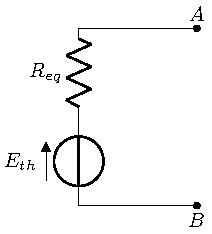
\includegraphics{rappresentazione-thevenin.pdf}}%
    \qquad
    \subfloat[\centering Forma Norton]{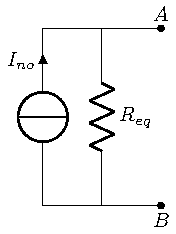
\includegraphics{rappresentazione-norton.pdf}}%
    \caption{Rappresentazioni Equivalenti di una Rete Adinamica}%
    \label{fig:rappresentazioni-equivalenti}
\end{figure}
\noindent
Le relazioni che legano i due circuiti equivalenti sono semplicemente:
$$I_{NO} = \frac{E_{TH}}{R_{TH}}$$ $$R_{NO} = R_{TH}$$
\subsection{Teorema del massimo trasferimento di potenza}
Grazie al \textbf{teorema di Thevenin} posso calcolare con il \textbf{teorema del massimo trasferimento di potenza}, la resistenza equivalente da attaccare alla rete per ottenere la \textbf{massima potenza erogabile}.
\begin{figure}[H] % Usa 'H' per forzare la posizione qui
    \centering % Centra l'immagine
    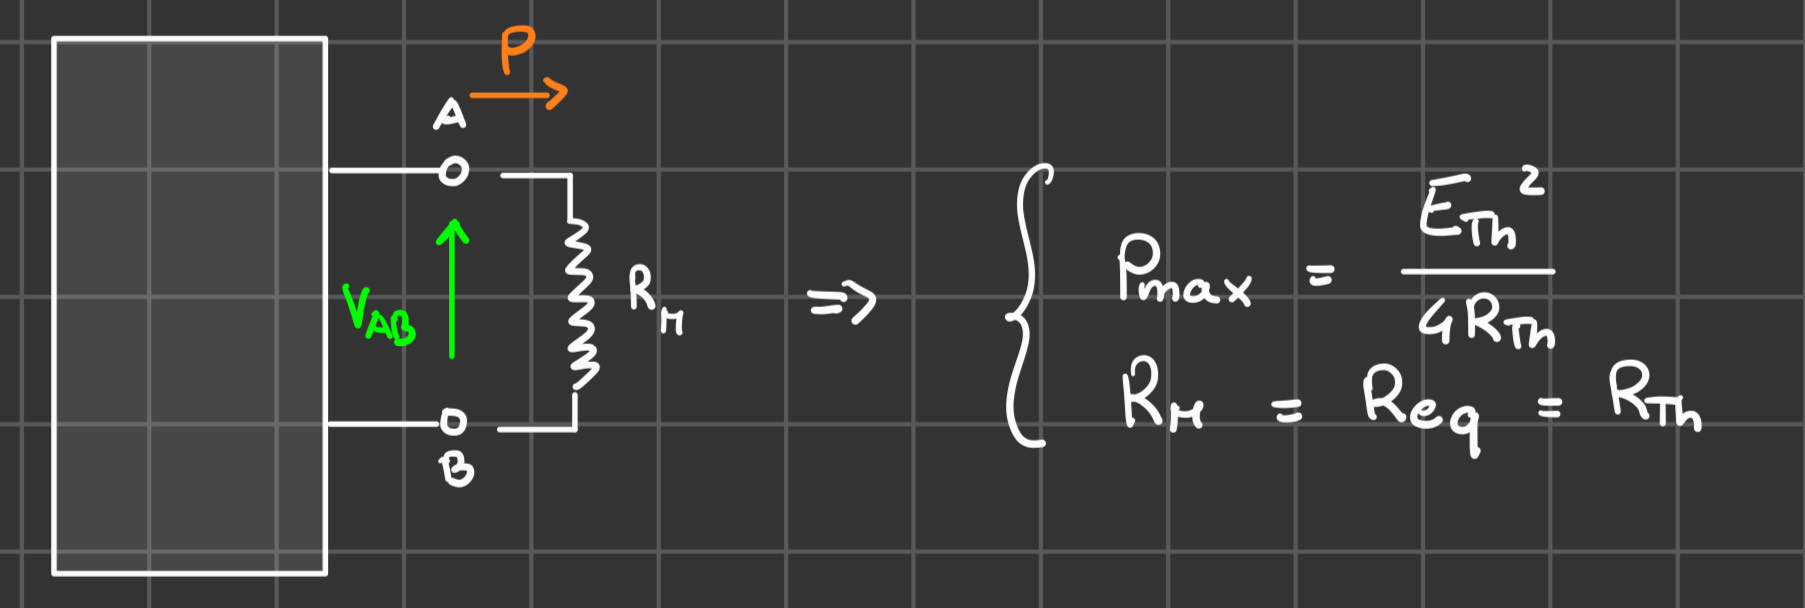
\includegraphics[width=10cm, height=3cm]{IMG_0868.jpeg} % Percorso dell'immagine
   % \caption{Datagram Header} % Didascalia per l'immagine
    \label{fig:immagine} % Etichetta per riferimento
\end{figure}
\noindent
Dimostrazione: \\
Calcoliamo la \textbf{tensione} tra i due punti A e B con il partitore di tensione: 
\begin{gather*}
    V_{AB}=\displaystyle\frac{R_M}{R_\mathrm{TH}+R_M}E_\mathrm{th}
\end{gather*}
\noindent
Calcoliamo la corrente che scorre sul Resistore $R_m$:
$$i=\frac{V_{AB}}{R_M}=\frac{E_{TH}}{R_{TH}+R_M}$$
Calcoliamo la potenza erogata sul resistore $R_m$: 
\begin{gather*}
    P=R_M*i^2=R_M\displaystyle\frac{E_\mathrm{th}^2}{(R_\mathrm{th}+R_M)^2}=\frac{E_\mathrm{th}^2}{\frac{R_\mathrm{th}^2}{R_M}+2R_\mathrm{th}+R_M}
\end{gather*}
\noindent
Per calcolare la potenza massima trasferibile da questo circuito, si considera la derivata della potenza in funzione della resistenza esterna. Per trovare il massimo, bisogna trovare il valore minimo del denominatore, per cui, si deriva solo il denominatore della funzione potenza $P(R_M)$:
\begin{gather*}
    \displaystyle\frac{\df}{\df R_M}\left(\frac{R_\mathrm{th}^2}{R_M}+2R_\mathrm{th}+R_M\right)=-\frac{R_\mathrm{th}^2}{R_M^2}+1=0\\
    R_M^2=R_\mathrm{th}^2,\,R>0\\
    R_M=R_\mathrm{th}\tageq
\end{gather*}
Per cui $P_{max}$:
$$P_{max}=\frac{R_ME_{TH}^2}{(R_{TH}+R_{M})^2}=R_{TH}\frac{E_{TH}^2}{4R_{TH}^2}=\frac{E_{TH}^2}{4R_{TH}}$$
\section{Reti Dinamiche}
\subsection{Carica e scarica del condensatore}
Si considera una rete, alimentata da un generatore di tensione a corrente continua, posto a valle di un commutatore ideale. Questo commutatore è un oggetto che permette 
di alterare la struttura del circuito commutando, per chiudere o aprire il circuito. Si considera uno stato iniziale dove il commutatore è aperto, ed all'istante $t=0$, 
con tempo di commutazione nulla, il circuito si chiude, e comincia a fluire corrente. Tra i due morsetti legati dal commutatore è presente il vuoto prima della chiusura, ed 
il cortocircuito dopo la commutazione: 
\begin{figure}[H]%
    \centering
    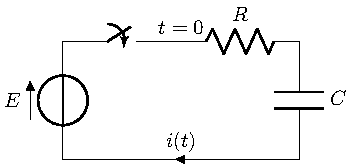
\includegraphics{circuito-rc-tempo-continuo.pdf}%
    \label{fig:circuito-rc}
\end{figure}
\noindent
La tensione assorbita dal resistore e dal condensatore sono quindi due grandezze variabili nel tempo. Non fluisce corrente all'interno del circuito prima della 
commutazione, per cui la corrente è una grandezza variabile nel tempo:
\begin{gather*}
    i(t)=\begin{cases}
        0&t\leq0^-\\
        i(t)&t>0^+
    \end{cases}
\end{gather*}
Per esprimere questo concetto, si considera nelle equazioni risolutive, la tensione generata come una funzione $e(t)$, che assume valore nullo per $t<0$, mentre un valore $E$ pari alla tensione erogata per $t>0$. Per rappresentare questa funzione si considera il segnale gradino unitario $u_{-1}(t)$:
\begin{equation*}
    e(t)=Eu_{-1}(t)
\end{equation*}
Si considerano le tensioni del resistore e del condensatore di polarità 
opposta rispetto al generatore di tensione. Applicando il principio di Kirchhoff alle tensioni si ottiene la seguente equazione:
\begin{gather*}
    e(t)=v_R(t)+v_C(t)
\end{gather*}
Si considera per ipotesi $t\geq0^+$, per non dover tenere conto del gradino unitario. Si inseriscono le leggi costitutive dei bipoli, e si ottiene la seguente equazione 
differenziale di primo ordine:
\begin{gather*}
    E=Ri+v_C\\
    E=RC\displaystyle\frac{\df v_C}{\df t}+v_C
\end{gather*}
Essendo un'equazione differenziale, la sua soluzione è formata dalla combinazione lineare tra l'integrale generale (soluzione dell'equazione omogenea) e l'integrale particolare, della stessa classe di funzioni della forzante:
\begin{equation*}
    v_C(t)=v_{Cg}(t)+v_{Cp}(t)
\end{equation*}
Si risolve l'equazione omogenea:
\begin{gather*}
    RC\displaystyle\frac{\df v_C}{\df t}+v_C=0
\end{gather*}
Per risolverla, calcoliamo il polinomio caratteristico associato, il quale corrisponde ad un'equazione lineare, con una sola radice:
\begin{gather*}
    RC\alpha+1=0\\
    \alpha=\displaystyle-\frac{1}{RC}\\
    v_{Cg}(t)=k_1e^{-\frac{1}{RC}t}
\end{gather*}
L'integrale particolare tiene conto della forzante inserita nel sistema, ed appartiene alla sua stessa classe di funzioni, per la proprietà della similarità. In questo caso, 
la forzante è una costante, per cui l'integrale particolare è:
\begin{gather*}
    v_{Cp}(t)=k_2
\end{gather*}
La soluzione completa è quindi data dalla somma di questi due integrali:
\begin{gather*}
    v_C(t)=k_1e^{-\frac{1}{RC}t}+k_2
\end{gather*}
Per trovare le costanti $k_1$ e $k_2$, si considera il problema di Cauchy, con le equazioni di vincolo fornite dal sistema. La carica del condensatore in $t=0^-$ è nota, 
per cui si può esprimere rispetto alle due costanti. La tensione erogata dal generatore, per tempi tendenti asintoticamente all'infinito, sarà assorbita 
completamente dal condensatore. Le equazioni di vincolo sono quindi:
\begin{gather*}
    \begin{cases}
        v_C(0^-)=k_1+k_2\\
        \displaystyle\lim_{t\to+\infty}v_C(t)=E=k_2
    \end{cases}\\
    \begin{cases}
        k_1=v_C(0^-)-E\\
        k_2=E
    \end{cases}\\
    \begin{cases}
        v_C(t)=(v_C(0^-)-E)e^{-\frac{1}{RC}t}+E&t\geq0^+\\
        i(t)=-\displaystyle\frac{1}{R}(v_C(0^-)-E)e^{-\frac{1}{RC}t} &t\geq0^+
    \end{cases}\tageq
\end{gather*}
Il condensatore si carica, quando la sua tensione al tempo $t=0^-$ è minore della tensione erogata dal generatore, mentre si scarica quando la sua tensione è maggiore della 
tensione erogata dal generatore:
\begin{gather*}
    \mbox{carica: }|v_C(0^-)|<|E|\\
    \mbox{scarica: }|v_C(0^-)|>|E|
\end{gather*}
\newpage
\noindent
Nel caso di semplice carica $v_c(0^-)=0$, le funzioni della tensione e della corrente diventano:
\begin{gather*}
    v_C(t)=E\left(1-e^{-\frac{1}{RC}t}\right)u_{-1}(t)\\
    i(t)=\displaystyle\frac{E}{R}e^{-\frac{1}{RC}t}
\end{gather*}
Essendo la grandezza RC un tempo, la definiamo come il tempo caratteristico $\tau$:
$$\tau=RC$$
\begin{figure}[H]%
    \centering
    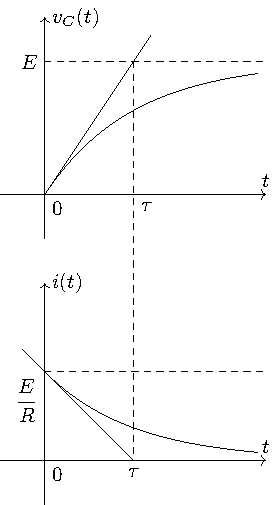
\includegraphics{andamento-circuito-rc.pdf}%
    \caption{Andamento delle Grandezze di un Circuito RC nel Tempo}
    \label{fig:andamento-circuito-rc}
\end{figure}
\newpage
\subsection{Carica e scarica dell'induttore}
Il duale della carica o scarica di un condensatore, è il caso della carica o scarica dell'induttore. In questo caso poiché è presente un generatore di corrente, e non 
può essere inserito a vuoto, il commutatore crea due circuiti chiusi, in modo che il generatore di corrente non sia mai collegato a vuoto:
\begin{figure}[H]%
    \centering
    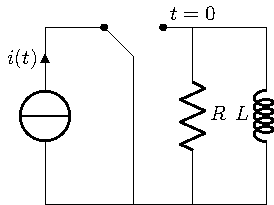
\includegraphics{circuito-rl-tempo-continuo.pdf}%
    \label{fig:circuito-rl}
\end{figure}
\noindent
Si considera il generatore di corrente continua, e per il principio di Kirchhoff alle 
correnti si ottiene la seguente equazione:
\begin{gather*}
    i(t)-Gv(t)-i_L(t)=0
\end{gather*}
Si considera la legge costitutiva dell'induttore:
\begin{gather*}
    v=L\displaystyle\frac{\df i_L(t)}{\df t}\\
    i(t)=GL\displaystyle\frac{\df i_L(t)}{\df t}+i_L(t)
\end{gather*}
Si considera il commutatore ideale, di tempo di commutazione istantaneo in $t=0$, per cui la corrente passante erogata corrisponde a:
\begin{gather*}
    i(t)=Iu_{-1}(t)
\end{gather*}
Si considera per ipotesi $t\geq0^+$, per non dover tenere conto del gradino unitario. Si inseriscono le leggi costitutive dei bipoli, e si ottiene la seguente equazione differenziale di primo ordine:
\begin{gather*}
    GL\displaystyle\frac{\df i_L}{\df t}+i_L=I\\
\end{gather*}
Essendo un'equazione differenziale, la sua soluzione è formata dalla combinazione lineare tra l'integrale generale (soluzione dell'equazione omogenea) e l'integrale particolare, della stessa classe di funzioni della forzante:
\begin{equation*}
    i_L(t)=i_{Lg}(t)+i_{Lp}(t)
\end{equation*}
Si risolve l'equazione omogenea:
\begin{gather*}
    GL\displaystyle\frac{\df i_L(t)}{\df t}+i_L(t)=0
\end{gather*}
Per risolverla, calcoliamo il polinomio caratteristico associato, il quale corrisponde ad un'equazione lineare, con una sola radice:
\begin{gather*}
     GL\alpha+1=0\\
  \alpha=\displaystyle-\frac{1}{GL}\\
  i_{Lg}(t)=k_1e^{-\frac{1}{GL}t}\\
\end{gather*}
L'integrale particolare tiene conto della forzante inserita nel sistema, ed appartiene alla sua stessa classe di funzioni, per la proprietà della similarità. In questo caso, 
la forzante è una costante, per cui l'integrale particolare è:
\begin{gather*}
    i_{Lp}(t)=k_2
\end{gather*}
La soluzione completa è quindi data dalla somma di questi due integrali:
\begin{gather*}
    i_L(t)=k_1e^{-\frac{1}{GL}t}+k_2
\end{gather*}
Per trovare le costanti $k_1$ e $k_2$, si considera il problema di Cauchy, con le equazioni di vincolo fornite dal sistema. Si inserisce la memoria dell'induttore, ed il caso per il tempo tendente asintoticamente all'infinito, dove tutta la corrente erogata dal generatore si trova nell'induttore:
\begin{gather*}
    \begin{cases}
        i_L(0^-)=k_1+k_2\\
        \displaystyle\lim_{t\to\infty}i_L(t)=I=k_2
    \end{cases}\\
    \begin{cases}
        k_1=i_L(0^-)-I\\
        k_2=I
    \end{cases}
\end{gather*}
Le funzioni della tensione e della corrente nel tempo sono quindi:
\begin{gather}
    \begin{cases}
        i_L(t)=(i_L(0^-)-I)e^{-\frac{1}{GL}t}+I\\
        v(t)=\displaystyle-\frac{1}{G}\cancel{\frac{L}{L}}(i_L(0^-)-I)e^{-\frac{1}{GL}t}
    \end{cases}
\end{gather}
Per cui si individuano le due situazioni di carica e scarica dell'induttore:
\begin{gather*}
    \mbox{carica: }|i_L(0^-)|<|I|\\
    \mbox{scarica: }|i_L(0^-)|>|I|
\end{gather*}
\newpage
\noindent
Nel caso semplice di carica $i_L(0^-)=0$, le funzioni della corrente e della tensione diventano:
\begin{gather*}
    i_L(t)=I\left(1-e^{-\frac{1}{GL}T}\right)\\
    v_L(t)=\displaystyle\frac{I}{G}e^{-\frac{1}{GL}t}
\end{gather*}
Essendo la grandezza GL un tempo, la definiamo come il tempo caratteristico $\tau$:
$$\tau=GL$$
\begin{figure}[H]%
    \centering
    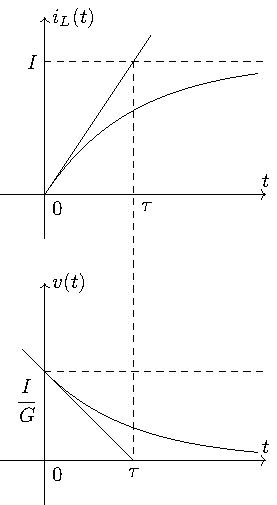
\includegraphics{andamento-circuito-rl.pdf}%
    \caption{Andamento delle Grandezze di un Circuito RL nel Tempo}
    \label{fig:andamento-circuito-rl}
\end{figure}
\newpage
\subsection{Circuiti in regime sinusoidale e fasori}
Si considera ora una forzante sinusoidale, e per rappresentarla si adopera una rappresentazione tramite i numeri complessi. Riscriviamo le equazioni di tensione e di corrente utilizzando le formule di Eulero.
\begin{gather*}
    v(t)=V_Msin(\omega t+ \alpha) = V_M \frac{1}{2j}(e^{j(\omega t+ \alpha)} - e^{-j(\omega t+ \alpha)})\\
    i(t) =I_Msin(\omega t+ \beta) = I_M \frac{1}{2j}(e^{j(\omega t+ \beta)} - e^{-j(\omega t+ \beta)})
\end{gather*}
Si definisce il fasore, della data forzante, come il numero complesso che codifica il valore di picco e la fase:
\begin{gather*}
    \overline{V}= \frac{V_Me^{j\alpha}}{2j},  \overline{I} = \frac{I_Me^{j\beta}}{2j}
\end{gather*}
Tramite i fasori si può esprimere la forzante sinusoidale come una combinazione lineare di esponenziali, moltiplicati per coefficienti complessi:
\begin{gather*}
    v(t)= V_M \frac{1}{2j}(e^{j(\omega t+ \alpha)} - e^{-j(\omega t+ \alpha)})=\overline{V}e^{j\omega t}- \overline{V*}e^{-j\omega t}\\
    i(t) = I_M \frac{1}{2j}(e^{j(\omega t+ \beta)} - e^{-j(\omega t+ \beta)})=\overline{I}e^{j\omega t}- \overline{I*}e^{-j\omega t}
\end{gather*}
Considerando i fasori: $\overline{V}= V_Me^{j\alpha}, \overline{I}= I_Me^{j\beta}$
\begin{gather*}
    v(t) = \frac{\overline{V}e^{j\omega t}- \overline{V*}e^{-j\omega t}}{2j},i(t)= \frac{\overline{I}e^{j\omega t}- \overline{I*}e^{-j\omega t}}{2j}
\end{gather*}
\subsection{Fasori nei circuiti RLC con forzante sinusoidale}
Si considera un generatore di tensione sinusoidale, inserito in un circuito RLC serie:
\begin{figure}[H]%
    \centering
    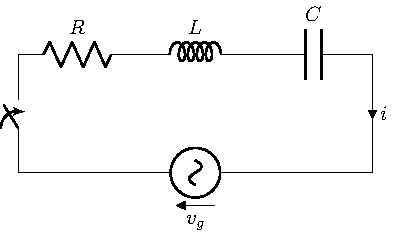
\includegraphics{circuito-rlc-serie-sinsusoide.pdf}%
    \label{fig:circuito-rlc-serie-sinusoide}
\end{figure}
\noindent
Dove la tensione erogata dal generatore è una funzione sinusoidale:
\begin{gather*}
    V_g(t)=V_msin(\omega t + \gamma)
\end{gather*}
Per il principio di Kirchoff alle tensioni, si ottiene la stessa equazione differenziale di un circuito RLC con tensione erogata costante. L'unico componente della soluzione totale della tensione che differisce è l'integrale particolare, poichè deve appartenere alla stessa classe delle funzioni della forzante:
\begin{gather*}
\begin{cases}
    v_g(t)=Ri(t)+\displaystyle L\frac{\df i(t)}{\df t}+v_C(t)\\
        i_C(t)=\displaystyle C\frac{\df v_C(t)}{\df t}
\end{cases}
\end{gather*}
Per la proprietà di similarità l'integrale particolare è anch'esso una sinusoide:
\begin{gather*}
    v_{Cp}(t)=V_M\sin(\omega t+\theta)\\
    v_{Cp}(0^-)=V_M\sin(\theta)
\end{gather*}
Poichè l'evoluzione libera tende a valori trascurabili, in un sistema asintoticamente stabile, per valori di tempo sufficientemente elevati, si analizza solo la risposta a regime permanente, ovvero l'integrale particolare, nel dominio dei fasori. Consideriamo quindi la risposta a regime permanente della tensione e della corrente $i_p(t)$:
\begin{gather*}
    i_p(t)=I_M\sin(\omega t+\beta)
\end{gather*}
Dove $I_M$ è la corrente massima e $\beta$ è la fase della corrente sinusoidale. Si vuole confermare se sia possibile applicare un approccio algebrico estendendo il teorema di Ohm solo sulla risposta a regime. Si vuole esprimere la tensione rispetto alla corrente a regime $i_p$:
\begin{gather*}
    v_{Cp}(t)=\displaystyle\frac{1}{C}\int_{0}^{t}i_p(\tau)\df\tau+v_C(0^-)
\end{gather*}
Poichè si analizza un tempo molto distante dal transitorio, non si può considerare la memoria $v_c(0-)$. Notiamo quindi che non si può proseguire per questa strada dato che l'integrale definito risulterebbe in una costante, mentre per similarità sappiamo che la risposta forzata dev'essere obbligatoriamente una sinusoide. Dobbiamo quindi cambiare dominio. Ricordando che nel dominio dei fasori:
\begin{gather*}
    i_p(t)=\displaystyle\frac{\overline{I}e^{j\omega t}-\overline{I}^*e^{-j\omega t}}{2j}\\
    v_{g}(t)=\displaystyle\frac{\overline{V}_ge^{j\omega t}-\overline{V}_g^*e^{-j\omega t}}{2j}\\
\end{gather*}
Portiamo $v_g(t)$ (vedi parentesi graffa) nel dominio dei fasori.
Per il principio di identità dei polinomi $\overline{V_g}$ sarà uguale a tutto ciò che moltiplica $\frac{e^{j\omega t}}{2j}$ (vale anche per il coniugato):
\begin{gather*}
    \overline{V_g} = R\overline{I} + j\omega L \overline{I} + \frac{1}{j\omega C}\overline{I}=[R + j(\omega L - \frac{1}{\omega C}]\overline{I}
\end{gather*}
Definendo quindi l'impedenza z:
\begin{gather*}
    z=R + j(\omega L - \frac{1}{\omega C})
\end{gather*}
E la legge di Ohm complessa:
\begin{gather*}
    \overline{V_g}=z\overline{I}
\end{gather*}
\newpage
\subsection{Studio l'impedenza al variare di w nei circuiti RLC serie}
Si considera un circuito RLC serie con generatori isofrequenziali, esprimendo l'impedenza in funzione della pulsazione:
\begin{gather}
    z(\omega)=R+j\displaystyle\left(\omega L-\frac{1}{\omega C}\right)\\
    |z(\omega)|=\displaystyle\sqrt{R^2+\left(\omega L-\frac{1}{\omega C}\right)^2}\\
    \varphi(\omega)=\arctan\left(\displaystyle\frac{\displaystyle\omega L-\frac{1}{\omega C}}{R}\right)
\end{gather}
Vogliamo esprimere la variazione dei valori dell'impedenza, al variare della pulsazione, considerando l'effetto di ogni componente singolarmente. La \textbf{parte reale del modulo} è sempre costante rispetto alla pulsazione, quindi il suo contributo è costante, mentre il suo contributo alla fase rimane nullo, poichè è puramente reale. L'\textbf{induttore} contribuisce linearmente all'aumento del modulo, mentre presenta sempre uno sfasamento di $\frac{\pi}{2}$. Il \textbf{condensatore} presenta un andamento iperbolico nel modulo, mentre presenta una sfasatura costante di $-\frac{\pi}{2}$.
\begin{figure}[H]%
    \centering
    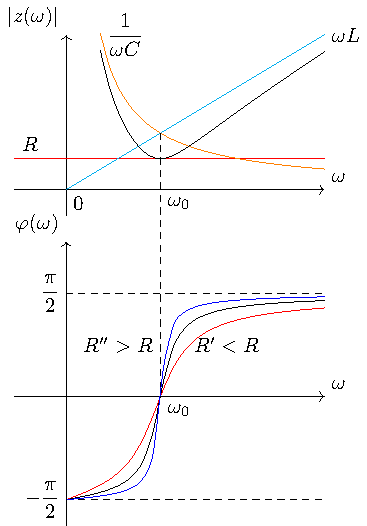
\includegraphics{andamento-impedenza-rlc-serie.pdf}%
    \caption{Andamento Modulo e Fase dell'Impedenza}%
    \label{fig:andamento-impedenza-rlc-serie}
\end{figure}
\noindent
Definiamo poi $\omega_0$ come la \textbf{pulsazione di risonanza}, che corrisponde a quella pulsazione la quale annulla la parte immaginaria dell'impedenza. Per $\omega<\omega_0$ abbiamo un comportamento ohmico-capacitivo e se $R=0$ abbiamo un comportamento puramente capacitivo, per $\omega>\omega_0$ abbiamo un comportamento ohmico-induttivo e se $R=0$ abbiamo un comportamento puramente induttivo. Per quanto riguarda la fase:\\
$$Per \qquad\omega->+\infty \quad \omega L>>\frac{1}{\omega C}$$
La fase dell'impedenza tende alla fase dell'induttanza $\varphi_z(\omega)=\frac{\pi}{2}$.
$$Per \qquad\omega=\omega_0$$
La fase è $\varphi_z(\omega)=0$
$$Per \qquad\omega->0 \quad \frac{1}{\omega C}>>\omega L$$
Di conseguenza la fase dell'impedenza tende alla fase del condensatore $\varphi_z(\omega)=-\frac{\pi}{2}$.
\subsection{Potenza in regime permanente sinusoidale}
Si vuole calcolare la potenza erogata da un generico lato, attraversato da una corrente sinusoidale e connesso ai due poli ad una tensione anch'essa sinusoidale:
\begin{gather*}
    v(t)=V_M\sin(\omega t+\gamma)\\
    i(t)=I_M\sin(\omega t+\gamma)
\end{gather*}
Si calcola la potenza istantanea erogata dal lato esprimendo le sinusoidi in forma euleriana:
\begin{gather*}
    i_p(t)=\displaystyle\frac{\overline{I}e^{j\omega t}-\overline{I}^*e^{-j\omega t}}{2j}\\
    v_{g}(t)=\displaystyle\frac{\overline{V}_ge^{j\omega t}-\overline{V}_g^*e^{-j\omega t}}{2j}\\
    p(t)=v(t)i(t)=\displaystyle\frac{\overline{V}e^{j\omega t}-\overline{V}^*e^{-j\omega t}}{2j}\frac{\overline{I}e^{j\omega t}-\overline{I}^*e^{-j\omega t}}{2j}\\
    \displaystyle-\frac{1}{4}\left(\overline{V}\overline{I}e^{2j\omega t}-\overline{V}\overline{I}^*-\overline{V}^*\overline{I}+\overline{V}^*\overline{I}^*e^{-2j\omega t}\right)
    =-\frac{1}{2}\frac{\overline{V}\overline{I}e^{2j\omega t}-(\overline{V}\overline{I})^*e^{-2j\omega t}}{2}+\frac{1}{2}\frac{\overline{V}\overline{I}^*+\overline{V}^*\overline{I}}{2}
\end{gather*}
Distinguiamo quindi una parte costante e una parte variabile nel tempo.
\begin{gather*}
    \overline{VI}=V_MI_Me^{j(\gamma+\beta)}\\
     (\overline{VI})^*=V_MI_Me^{-j(\gamma+\beta)}\\
    \overline{V}\overline{I}^*=V_MI_Me^{j(\gamma-\beta)}\\
    \overline{V}^*\overline{I}=V_MI_Me^{-j(\gamma-\beta)}\\
    \gamma-\beta=\varphi\\
    \gamma+\beta=2\gamma-\varphi
\end{gather*}
Si applicano queste sostituzioni appena definite, e si esprime in questo modo la potenza istantanea di un generico lato come la somma di due sinusoidi, una funzione nel tempo, 
mentre l'altra costante:
\begin{gather*}
    p(t)=\displaystyle-\frac{1}{2}V_MI_M\frac{e^{j(2\gamma t+2\gamma-\varphi)}+e^{-j(2\gamma t+2\gamma-\varphi)}}{2}+\frac{1}{2}V_MI_M\frac{e^{j\varphi}+e^{-j\varphi}}{2}\\
    -\displaystyle\frac{1}{2}V_MI_M\cos(2\omega t+2\gamma-\varphi)+\frac{1}{2}V_MI_M\cos\varphi\\
    p_f(t)=-\displaystyle\frac{1}{2}V_MI_M\cos(2\omega t+2\gamma-\varphi)\\
    P=\displaystyle\frac{1}{2}V_MI_M\cos\varphi\tageq
\end{gather*}
La parte variabile nel tempo la definiamo come potenza fluttuante $p_f(t)$, mentre la seconda componente la chiamiamo potenza attiva P, e rappresenta il valor medio della potenza istantanea. Definiamo inoltre $cos(\varphi)$ come fattore di potenza, dove $\varphi$ è lo sfasamento tra tensione e corrente.\\
Definiamo ora i valori efficaci:
\begin{gather}
    \begin{cases}
        V_{eff}=\displaystyle\frac{V_{M}}{\sqrt{2}}\implies V_M=\sqrt{2}V_{\mathrm{eff}}\\
        I_{eff}=\displaystyle\frac{I_{M}}{\sqrt{2}}\implies I_M=\sqrt{2}I_{\mathrm{eff}}
    \end{cases}
\end{gather}
Che ci permetteranno di esprimere la potenza come:
\begin{gather*}
    p(t)=V_{eff}I_{eff}cos(\varphi) - V_{eff}I_{eff}\cos(2\omega t+2\gamma-\varphi)
\end{gather*}
Rappresentiamo su un grafico le due funzioni della potenza:
\begin{figure}[H]
    \centering
    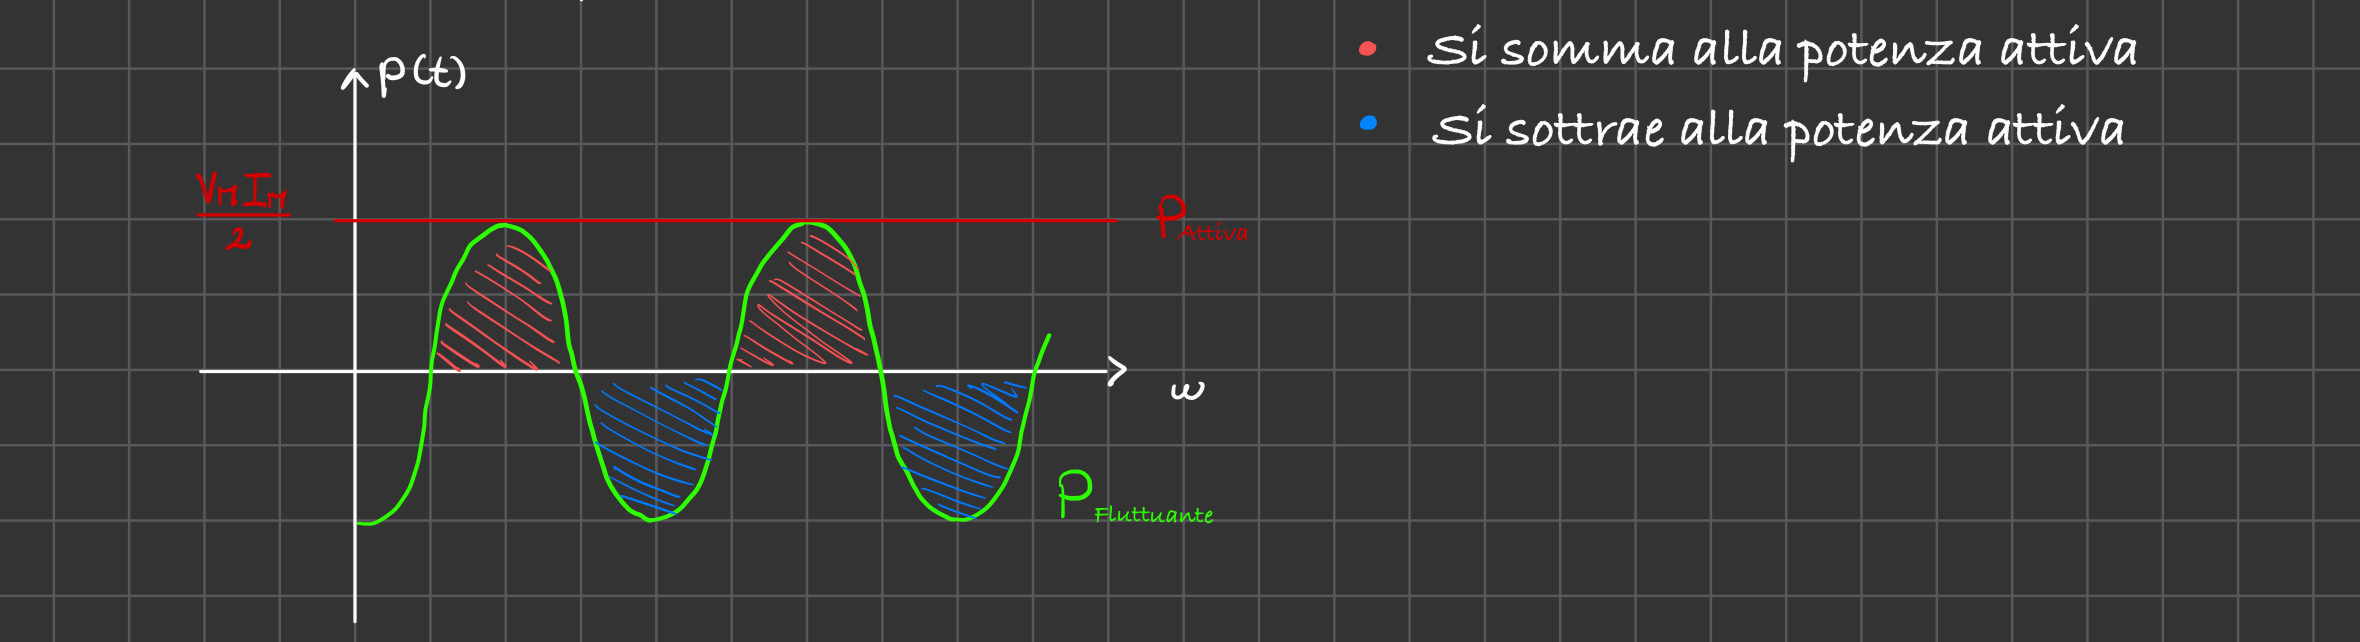
\includegraphics[width=15cm, height=6cm]{IMG_0869.jpeg}
    \label{fig:Potenza attiva e passiva}
\end{figure}
\noindent
Le zone in rosso, si trovano sull'asse positivo e sono quegli intervalli di tempo in cui viene assorbita potenza, che quindi si va ad aggiungere alla potenza attiva. Le zone in blu, corrispondono a quegli intervalli di tempo in cui viene generata potenza che si va a sottrarre a quella attiva.\\
Definiamo la potenza complessa come:
$$P_c=\overline{VI^*}$$
La quale è composta, da una parte reale, la potenza attiva e una parte immaginaria, la potenza reattiva.
\begin{gather*}
    P_c= P + jQ\\
    P = |P_c|\cos(\varphi)\\
    Q= |P_c|sin(\varphi)
\end{gather*}
Se la potenza reattiva è positiva, allora corrisponde a potenza assorbita dal lato, se è negativa, allora la potenza viene erogata dal lato.
\newpage
\subsection{Teorema del massimo trasferimento di potenza per reti dinamiche}
Nel caso di reti senza memoria, si ottiene la massima potenza, quando la resistenza di carico equivale alla resistenza equivalente di Thevenin. Si considera ora un generico circuito dinamico, accessibile dall'esterno da due morsetti:
\begin{figure}[H]%
    \centering
    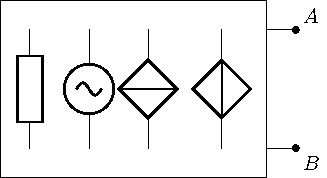
\includegraphics{generico-circuito-dinamico.pdf}%
    \label{fig:generico-circuito-dinamico}
\end{figure}
\noindent
Si vuole determinare la massima potenza attiva estraibile da un qualsiasi circuito dinamico, in funzione dell'impedenza. Tutto ciò che è stato trattato nelle reti adinamiche 
può essere riportato in una situazione dinamica nel dominio di fasori considerando impedenze e generatori dinamici. Per cui si può esprimere un qualsiasi circuito 
tramite il teorema di Thevenin a regime sinusoidale, con un generatore di tensione sinusoidale che presenta un fasore di tensione $\overline{E}_th$ equivalente al fasore 
di tensione misurato a vuoto tra i due morsetti $\overline{V}_{AB0}$, ed un'impedenza equivalente $z_\mathrm{eq}$, misurata rendendo passiva la rete. Si considera quindi un'impedenza 
di carico $z_C$, in modo da avere la massima potenza attiva:
\begin{figure}[H]%
    \centering
    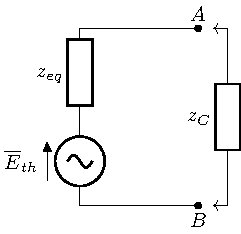
\includegraphics{rappresentazione-thevenin-fasori-carico.pdf}%
    \label{fig:rappresentazione-thevenin-fasori-carico}
\end{figure}
\noindent
La corrente erogata sul carico corrisponde a:
\begin{gather*}
    \overline{I}=\displaystyle\frac{\overline{E}_\mathrm{th}}{z_\mathrm{eq}+z_C}
\end{gather*}
Si può considerare la parte reale ed immaginaria dell'impedenza Thevenin e di carico:
\begin{gather*}
    \overline{I}=\displaystyle\frac{\overline{E}_\mathrm{th}}{(R_\mathrm{eq}+R_{C})+j(X_\mathrm{eq}+X_C)}
\end{gather*}
La potenza complessa può essere espressa come il prodotto tra l'impedenza ed il quadrato del valore efficace della corrente:
\begin{gather*}
    \dot P_C=zI^2=RI^2+jXI^2
\end{gather*}
Per cui per ottenere la potenza attiva assorbita dall'impedenza di carico si considera:
\begin{gather*}
    P_C=R_C|\overline I|^2=R_C\displaystyle\frac{E_\mathrm{th}^2}{(R_\mathrm{eq}+R_C)^2+(X_\mathrm{eq}+X_C)^2}
\end{gather*}
Ora effettuiamo un ragionamento in ambito Elettrotecnico, analogo a quello effettuato per determinare il massimo trasferimento di potenza in una rete adinamica. Si considera il massimo della potenza, quando si ha masssimizzato la corrente, a parità di resistenza. Per tornare a questa situazione analoga, bisogna diminuire il contributo della reattanza X. Per cui si considera la reattanza di carico:
\begin{gather*}
    X_C=-X_\mathrm{eq}\\
    X_\mathrm{tot}=0
\end{gather*}
Avendo una reattanza nulla ci si trova in una condizione di risonanza. Per cui si inserisce un'impedenza esterna per risonare il circuito. Questa è quindi la prima 
condizione per il teorema. In questa situazione dove il circuito si comporta come una rete adinamica, vale il teorema del massimo trasferimento di potenza, dimostrato 
per le reti adinamiche $R_C=R_\mathrm{eq}$. 
Per cui per estrarre la massima potenza da una rete dinamica bisogna inserire un'impedenza di carico pari al coniugato dell'impedenza equivalente del circuito:
\begin{gather}
    z_C=z_\mathrm{eq}^*
\end{gather}
\newpage
\section{Semiconduttori, Diodi e Transistor}
\subsection{Diodi: cosa sono, polarizzazione diretta e inversa}
\textbf{Un diodo a giunzione}, è un componente elettronico passivo, viene realizzato accostando tra di loro due regioni N e P. Una \textbf{regione P} è una regione identificata da un semiconduttore il quale è stato drogato con atomi del terzo gruppo diventando carico positivamente. Una \textbf{regione N} è una regione identificata da un semiconduttore il quale è stato drogato con atomi del quinto gruppo diventando carico negativamente.
\begin{figure}[H]%
    \centering
    \subfloat[\centering  Direttamente Polarizzato]{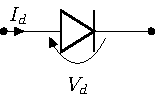
\includegraphics{diodo-direttamente-polarizzato.pdf}}%
    \qquad
    \subfloat[\centering Inversamente Polarizzato]{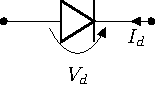
\includegraphics{diodo-inversamente-polarizzato.pdf}}%
    \caption{Diodo a Giunzione}
    \label{fig:diodo-giunzione}
\end{figure}
\noindent
L'\textbf{anodo} identifica il drogaggio P, mentre il \textbf{catodo} identifica il drogaggio N. 
Quando il diodo è polarizzato direttamente vi è una conduzione significativa. 
Invece se è presente una polarizzazione inversa ricade nella corrente inversa di saturazione, fino a quando non viene inserito un campo elettrico 
abbastanza elevato in grado da mandare in ``breakdown'' il diodo.  
La tensione inversa non può quindi superare questa tensione limite di ``breakdown''. Il comportamento del diodo, oggetto non lineare, può essere analizzato applicando una linearizzazione a tratti:
\begin{figure}[H]%
    \centering
    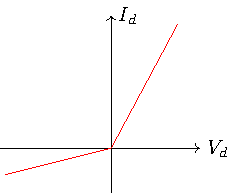
\includegraphics{diodo-linearizzazione.pdf}%
    \label{fig:diodo-linearizzazione}
\end{figure}
\noindent
In questo modo si analizza la corrente di conduzione in funzione ai capi del diodo. 
Per cui nel caso di \textbf{polarizzazione diretta} si associa al diodo un valore di resistenza bassa, mentre nel caso di \textbf{polarizzazione inversa}, la 
resistenza associata al diodo è molto elevata. Questo valore di resistenza si riferisce al rapporto tra l'incremento della tensione e della corrente. 
Questo modello viene perfezionato inserendo una piccola tensione di un valore di tensione di $V_{\gamma}\approx0.6$, prima della quale il diodo non 
presenta una corrente di conduzione, poiché rappresenta la tensione che rimane ai capi del diodo ed impedisce la conduzione.\newpage 
\noindent
L'andamento della corrente di conduzione di un diodo viene quindi descritto dalla seguente curva caratteristica: 
\begin{figure}[H]%
    \centering
    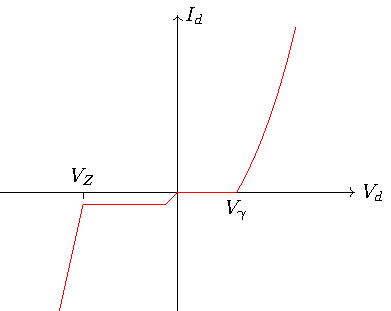
\includegraphics{andamento-diodo.pdf}%
    \caption{Curva caratteristica del Diodo}
    \label{fig:andamento-diodo}
\end{figure}
\noindent
La \textbf{curva caratteristica} esprime graficamente l'andamento della corrente I, al variare della tensione tra anodo e catodo V per un generico diodo. Per \textbf{tensioni V positive} la giunzione è polarizzata direttamente e la corrente fluisce dall'anodo al catodo.
La corrente di conduzione cresce molto rapidamente rispetto a piccoli incrementi di tensione in polarizzazione diretta. Per valori di V compresi fra 0 e V, la corrente assume valori trascurabili. Per \textbf{tensioni V negative} la giunzione è polarizzata inversamente e la corrente inversa di saturazione fluisce dal catodo all'anodo. In interdizione la corrente rimane costante al valore della corrente inversa di saturazione, fino ad un valore $V_Z$, \textbf{tensione Zener}, valore minimo dopo il quale il 
diodo vada in ``breakdown", ed entra in conduzione in modo non convenzionale, generalmente distruggendo il dispositivo. 
\subsection{Diodo Zener}
I \textbf{diodi Zener} sono diodi costruiti per funzionare nella regione di breakdown, ovvero in prossimità della tensione Zener $V_z$. Si costruisce questo oggetto per mantenere costante un valore della tensione (inversa) a prescindere dal valore della corrente, per cui si comporta come uno \textbf{stabilizzatore di tensione}. La resistenza del diodo viene calcolata come rapporto tra l'incremento della corrente e della tensione, superata la tensione di Zener $V_z$ il rapporto tenderà a infinito e trovandosi vicino al "breakdown", piccole variazioni di tensione provocano un elevata risposta in corrente, che potrebbe portare alla distruzione del componente. Un diodo Zener è costruito in modo da poter lavorare in polarizzazione inversa, il valore $V_z$ dipende dalla resistività del materiale delle sue giunzioni.
\begin{figure}[H]%
    \centering
    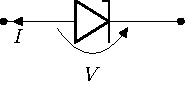
\includegraphics{diodo-zener.pdf}%
    \label{fig:diodo-zener}
\end{figure}
\subsection{Ponte di Graetz o Raddrizzatore a semionda}
Un ponte raddrizzatore a semionda è costituito da quattro diodi, i quali permettono il passaggio sia dalla semionda positiva che da quella negativa. 
\begin{figure}[H]%
    \centering
    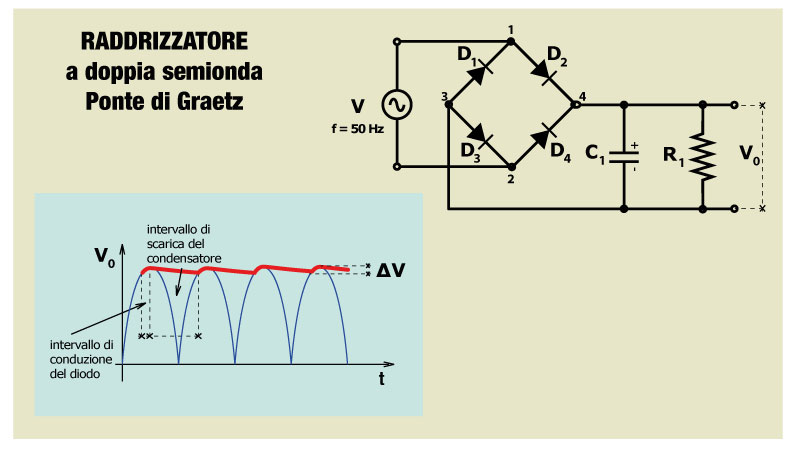
\includegraphics[width=15cm, height=6cm]{raddrizzatore-a-doppia-semionda.jpg}%
    \label{fig:ponte-graetz}
\end{figure}
\noindent
Il ponte di Graetz o raddrizzatore a doppia semionda lavora in questo 
modo: \\
• Sul terminale 1 c’è la semionda positiva e sul 2 quella negativa: 
la tensione verrà raddrizzata dai diodi D2 e D3. \\
• Sul terminale 1 c’è la semionda negativa e sul 2 quella positiva: 
la tensione verrà raddrizzata dai diodi D1 e D4. \\
Dall’uscita quindi del Ponte di Graetz si avranno le semionde positive con 
frequenza doppia, circa il 60$\%$ in più della frequenza del segnale 
all’ingresso del circuito. Si osservi che il valore di tensione in uscita è 
inferiore rispetto a quella di ingresso. Si può risolvere questo problema 
con un condensatore elettrolitico con un tempo di scarica sufficientemente 
lungo da consentire il livellamento della tensione di uscita e l’annullamento 
della pulsazione in uscita.
\newpage
\subsection{Porte Logiche OR e AND}
Le porte logiche sono dei componenti digitali che prendono un certo numero input e producono un output determinato da leggi note a priori che caratterizzano la porta.
\subsubsection{Operazione OR e NOR}
Si considera l'operazione OR e si vuole implementare questa porta logica tramite diodi, indicando gli ingressi e le uscite come 0 o 1 in base alla tensione. Un valore alto rappresenta un 1 logico, mentre un valore basso rappresenta uno 0 logico.
\begin{figure}[H]%
    \centering
    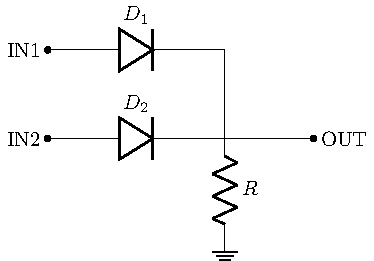
\includegraphics{circuito-or.pdf}%
    \label{fig:circuito-or}
\end{figure}
\noindent
Si considerano due generatori di tensione in input, collegati alla massa comune. A valle sono presenti due interruttori per ciascun input che chiudono il circuito con un generatore, oppure con un cortocircuito. Se il circuito viene chiuso con un cortocircuito, il diodo relativo a quell'input non è polarizzato e non conduce, per cui rappresenta uno zero logico. Se il circuito viene chiuso con un generatore di tensione, il diodo associato a quell'input viene polarizzato e conduce. Se almeno uno dei due diodi è in conduzione possono alimentare la resistenza R che aumenta la tensione fino al valore in ingresso alla rete.
\begin{figure}[H]%
    \centering
    \subfloat[\centering OR]{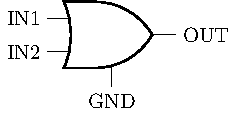
\includegraphics{or-gate.pdf}}%
    \qquad
    \subfloat[\centering NOR]{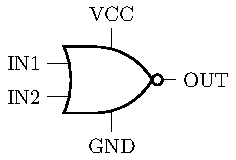
\includegraphics{nor-gate.pdf}}%
    \caption{Porte OR e NOR}
    \label{fig:porte-or-nor}
\end{figure}
\newpage
\subsubsection{Operazione AND}
Si considera il seguente circuito per descrivere la logica AND:
\begin{figure}[H]%
    \centering
    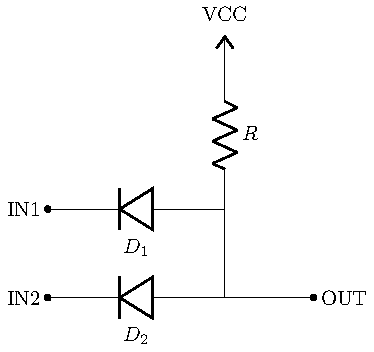
\includegraphics{circuito-and.pdf}%
    \label{fig:circuito-and}
\end{figure}
\noindent
Invece di indicare il generatore di tensione, generalmente si inserisce VCC con un certo valore di tensione, misurata rispetto al comune, per indicare la presenza del generatore di tensione. Se vengono inseriti due generatori di tensioni, che erogano tensione pari a VCC, allora mandano i due diodi in interdizione, per cui si ottiene un 1 logico in output. Invece per ottenere uno zero logico in uscita, è sufficiente uno solo dei due diodi in conduzione, per cui questo circuito descrive la logica AND.
\begin{figure}[H]%
    \centering
    \savebox{\tempbox}{\hbox{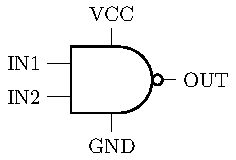
\includegraphics{nand-gate.pdf}}} %% fix alingment
    \subfloat[valign=t][\centering AND]{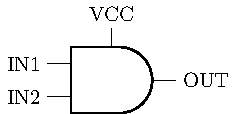
\includegraphics{and-gate.pdf}}%
    \qquad 
    \subfloat[valign=t][\centering NAND]{\usebox{\tempbox}}%
    \caption{Porte AND e NAND}
    \label{fig:porte-and-nand}
\end{figure}
\newpage
\subsection{Transistor}
Il \textbf{transistor o BJT ("Bipolar Junction Transistor")} è un componente 
elettronico, viene impiegato all'interno di circuiti integrati utilizzando 
per la sua costruzione il silicio, noto come materiale semiconduttore.
Il transistor viene anche chiamato \textbf{transistor bipolare} poichè in esso, il processo di 
conduzione coinvolge portatori di carica di entrambe le polarità, positiva e 
negativa. Questo lo distingue dai transistor ad effetto di campo JFET ("Junction Field Effect Transistor"), dove la conduzione vede 
coinvolti portatori di carica di un solo tipo, elettroni o lacune. I BJT sono transistor \textbf{controllati in corrente}, mentre i FET sono controllati in tensione. Un BJT è un \textbf{due-porte sbilanciato}, contenente un morsetto chiamato \textbf{base B}, un morsetto chiamato \textbf{collettore C} ed uno chiamato \textbf{emettitore E}. I transistor \textbf{PNP} o \textbf{NPN} sono costruiti collegando tre zone complementari in successione, per creare due giunzioni, la giunzione del collettore $J_C$ e la giunzione dell'emettitore $J_E$.
\begin{figure}[H]%
    \centering
    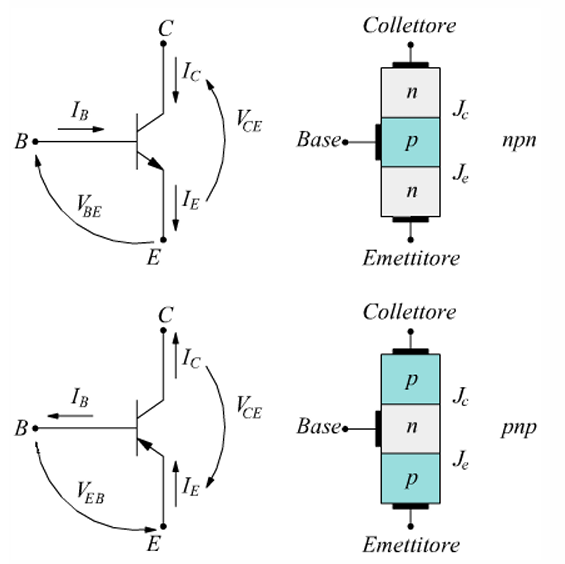
\includegraphics[width=10cm, height=6cm]{Screenshot 2025-02-15 145843.png}%
    \label{fig:Transistor NPN o PNP}
\end{figure}
\noindent
Andiamo ad analizzare il comportamento di un transistor:
\begin{figure}[H]%
    \centering
    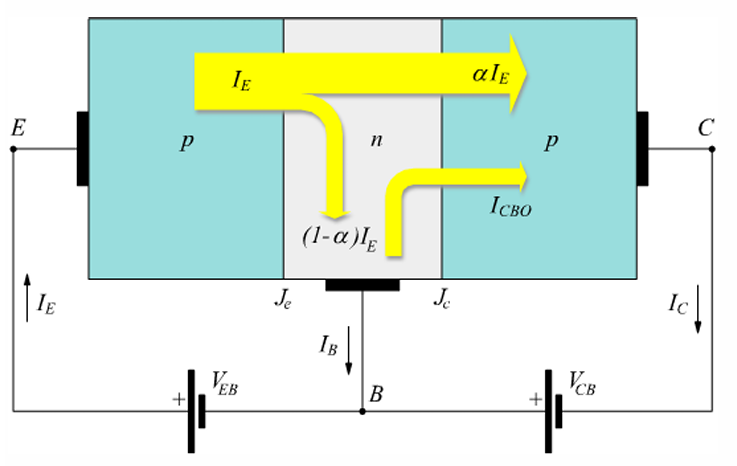
\includegraphics[width=10cm, height=5cm]{Screenshot 2025-02-15 152017.png}%
    \label{fig:Transistor NPN o PNP}
\end{figure}
\noindent
Se viene \textbf{polarizzato positivamente l'emettitore} rispetto alla base, le lacune della zona P, connessa all'emettitore, fluiscono verso zone a potenziale più basso. Se il \textbf{collettore} anch'esso viene \textbf{polarizzato} con un potenziale più basso rispetto alla base allora le lacune potranno fluire o verso la base o verso il collettore. Essendo la base dimensionalmente più piccola rispetto all'emettitore, le cariche che non sono andate in base, finiscono verso il collettore che ha un potenziale ancora più basso. Definiamo il \textbf{fattore di trasferimento di corrente} $\alpha$ come la frazione di lacune iniettate dall'emettitore che raggiunge il collettore senza ricombinarsi nella base, per cui possiamo esprimere le correnti $I_E$ (corrente misurata all'emettitore) , $I_C$ (corrente di collettore) e $I_B$ (corrente di base):
\begin{gather*}
    I_B=(1-\alpha)I_E\\
    I_C=\alpha I_E
\end{gather*}
Per la legge del tri-polo si ottiene la seguente relazione facilmente verificabile:
\begin{gather*}
    I_E=I_B+I_C
\end{gather*}
\subsection{Caratteristiche di ingresso e di uscita}
Si considera ora un circuito con un transistor NPN, il più usato, per studiare il comportamento non lineare del transistor:
\begin{figure}[H]%
    \centering    
    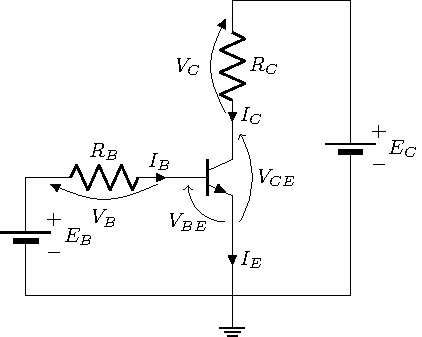
\includegraphics{circuito-bjt.pdf}%
    \label{fig:circuito-bjt}
\end{figure}
\noindent
Sono presenti due maglie, la maglia di base emettitore BE e la maglia di collettore emettitore CE. Sono connessi due generatori in continuo per mandare in polarizzazione il transistor.
\newpage
\subsubsection{Caratteristiche di ingresso}
Analizzando la maglia BE, le grandezze $I_B$ e $V_{BE}$ sono caratteristiche non lineari. Andando a graficare i valori di $I_B$ al variare di $V_{BE}$:
\begin{figure}[H]%
    \centering
    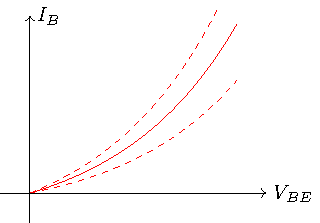
\includegraphics{andamento-base.pdf}%
    \label{fig:andamento-base}
\end{figure}
\noindent
Si rappresenta una famiglia di curve, associata ognuna ad un valore diverso di $V_{CE}$, in base alla pendenza della curva.
\subsubsection{Caratteristiche di uscita}
Analizzando la maglia CE, la corrente di collettore $I_C$ e la tensione collettore emettitore $V_{CE}$ sono anch'esse caratteristiche non lineari. Andando a graficare i valori di $I_C$ al variare di $V_{CE}$:
\begin{figure}[H]%
    \centering
    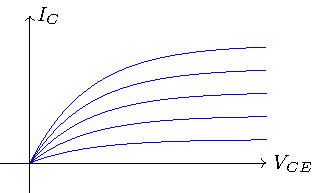
\includegraphics{andamento-collettore.pdf}%
    \label{fig:andamento-collettore}
\end{figure}
\noindent
Si rappresentano mediante una famiglia di curve associate a valori crescenti di corrente di base $I_B$.
\newpage
\subsection{Polarizzazione}
La polarizzazione del transistor, di fatto, viene ottenuta dal circuito precedente andando ad individuare sulle caratteristiche di uscita, l'intersezione fra la retta di carico e la curva di uscita corrispondente allo specifico valore di $V_{BE}$ in atto. Infatti applicando il principio di Kirchoff alle tensioni sulla maglia CE:
\begin{figure}[H]%
    \centering
    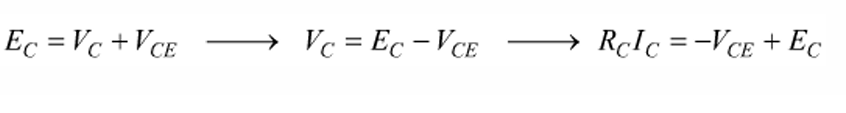
\includegraphics[width=13cm, height=2cm]{Screenshot 2025-02-17 125543.png}%
    \label{fig:Transistor NPN o PNP}
\end{figure}
\noindent
\begin{figure}[H]%
    \centering
    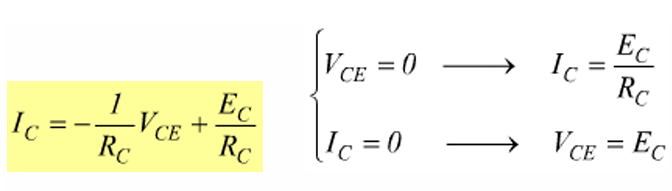
\includegraphics[width=13cm, height=3cm]{Screenshot 2025-02-17 125558.png}%
    \label{fig:Transistor NPN o PNP}
\end{figure}
\noindent
\begin{figure}[H]%
    \centering
    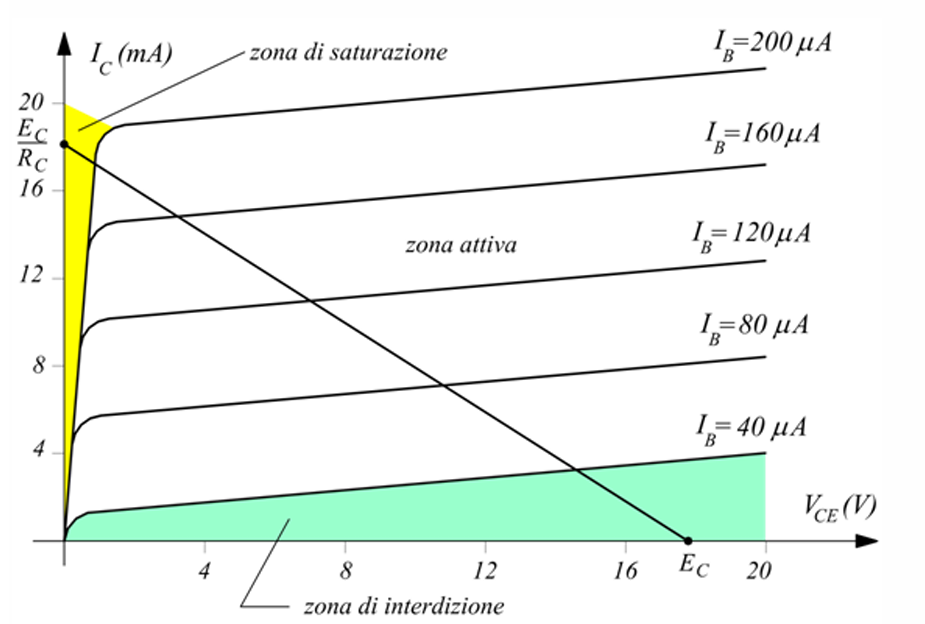
\includegraphics[width=9cm, height=5cm]{Screenshot 2025-02-17 125607.png}%
    \label{fig:Transistor NPN o PNP}
\end{figure}
\noindent
Distinguiamo quindi tre zone:\\
- La zona attiva: è la zona centrale delle caratteristiche di uscita, detta anche di funzionamento lineare.\\
- La zona di saturazione: con bassi valori di $V_{CE}$ in cui l'insieme delle curve di uscita tendono a confondersi in un unico tratto quasi verticale.\\
- La zona di interdizione: pressochè coincidente con l'asse delle ascisse in cui sia $I_B$ che $I_C$ hanno valori trascurabili.\\
Se si vuole usare il BJT come amplificatore quindi in modo lineare, il punto di lavoro deve essere scelto opportunamente all'interno della zona attiva. Se si vuole usare il BJT come interruttore il punto di lavoro può solo commutare fra la zona di interdizione e la zona di saturazione.
\subsection{Polarizzazione con partitore di base}
Nel circuito di polarizzazione precedente si nota la presenza di due batterie di alimentazione. Vogliamo ora utilizzare un solo generatore:
\begin{figure}[H]%
    \centering
    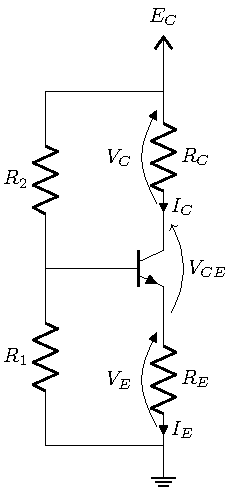
\includegraphics{bjt-polarizzazione.pdf}%
    \label{fig:bjt-polarizzazione}
\end{figure}
\noindent
Applichiamo il teorema di Thevenin e calcoliamo la tensione a vuoto con il partitore di tensione:
\begin{gather*}
    V_{BO}=E_C\displaystyle\frac{R_1}{R_1+R_2}
\end{gather*} 
\begin{figure}[H]%
    \centering
    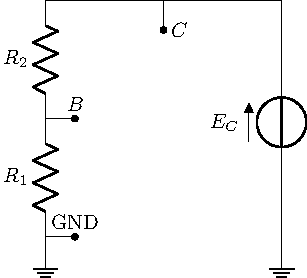
\includegraphics{bjt-tensione-thevenin.pdf}%
    \label{fig:bjt-tensione-thevenin}
\end{figure}
\noindent 
La resistenza di Thevenin si ottiene inserendo un cortocircuito al posto di $E_C$ e dato che $R_1$ e $R_2$ sono in parallelo si ottiene:
\begin{gather*}
    R_B=\displaystyle\frac{R_1R_2}{R_1+R_2}
\end{gather*}
\begin{figure}[H]%
    \centering
    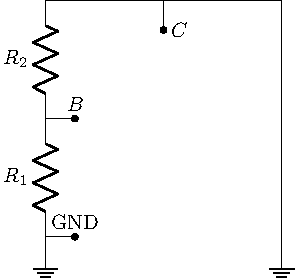
\includegraphics{bjt-resistenza-thevenin.pdf}%
    \label{fig:bjt-resistenza-thevenin}
\end{figure}
\noindent
Andiamo quindi a considerare la medesima analisi svolta per il circuito precedente, andando ad aggiungere una resistenza connessa all'emettitore:
\begin{figure}[H]%
    \centering
    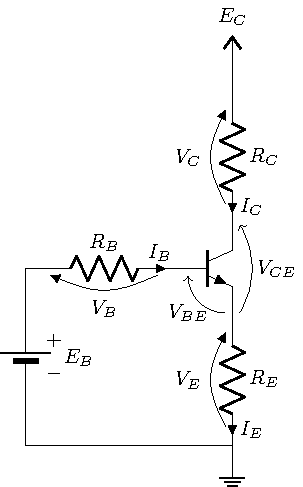
\includegraphics{bjt-circuito-polarizzazione.pdf}%
    \label{fig:bjt-circuito-polarizzazione}
\end{figure}
\noindent
Studiamo ora le due maglie, tenendo conto della resistenza inserita:
\begin{gather*}
    \mbox{BE: }E_B=R_BI_B+V_{BE}+R_EI_E\\
    \mbox{CE: }E_C=R_CI_C+V_{CE}+R_EI_E
\end{gather*}
Ricordando che $I_C=\alpha I_E \approx I_E$, otteniamo la seguente espressione:
\begin{gather*}
    E_C=R_CI_C+V_{CE}+R_EI_E=R_CI_C+V_{CE}+R_EI_C\\
    I_C=\displaystyle\frac{E_{C}}{R_C+R_E}-\frac{1}{R_C+R_E}V_{CE}
\end{gather*}
L'unica differenza è quindi la presenza della resistenza dell'emettitore al denominatore, invece della sola resistenza del collettore, ciò non 
provoca variazioni qualitative rispetto all'analisi effettuata considerando solamente la resistenza del collettore:
\begin{figure}[H]%
    \centering
    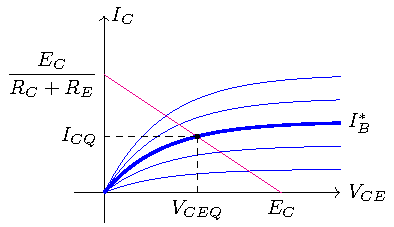
\includegraphics{andamento-collettore-emettitore.pdf}%
    \label{fig:andamento-collettore-emettitore}
\end{figure}
\subsection{Porte Logiche NOR e NAND}
Grazie al transistor BJT, possiamo costruire circuiti che rispettano la logica NOR e NAND. \\
Porta NOR:
\begin{figure}[H]%
    \centering
    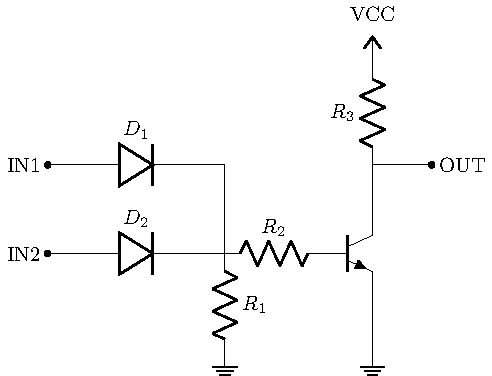
\includegraphics{circuito-nor.pdf}%
    \caption{Porta NOR}%
    \label{fig:circuito-nor}
\end{figure}
\noindent
Porta NAND:
\begin{figure}[H]%
    \centering
    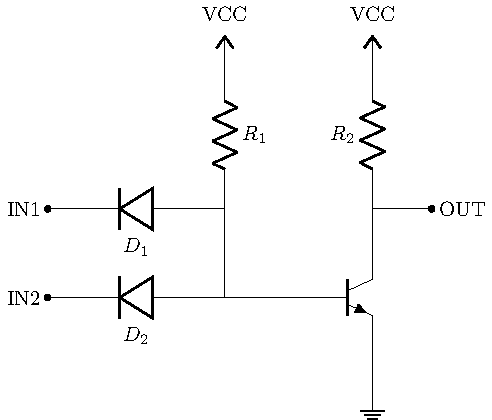
\includegraphics{circuito-nand.pdf}%
    \caption{Porta NAND}
    \label{fig:circuito-nand}
\end{figure}
\noindent
Il segnale in uscita dalla componente OR e AND, comanda un interruttore, formato da un transistor BJT.Se il transistor va in saturazione e 
conduce, se in entrata è presente un uno logico corrispondente ad un valore alto di tensione, realizza un cortocircuito tra il GND e 
l'output, producendo uno zero logico in uscita. Se è presente uno zero logico in entrata al transistor, il circuito è aperto, per cui la corrente 
di collettore non fluisce e ed il potenziale VCC esce in output, producendo un uno logico. 
\newpage
\subsection{Modello a parametri ibridi}
Questo modello, modella il comportamento del transistor nella regione attiva, in questa regione il transistor opera come amplificatore del segnale. Individuiamo tre zone, la zona di amplificazione, il generatore del segnale ed il carico del circuito:
\begin{figure}[H]%
    \centering
    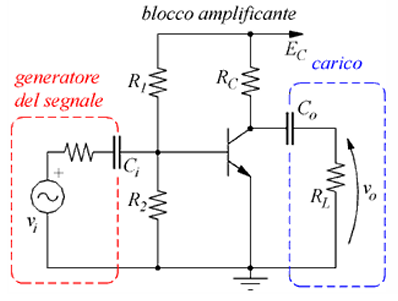
\includegraphics[width=9cm, height=5cm]{immagine_2025-02-18_134030203.png}%
    \label{fig:Transistor NPN o PNP}
\end{figure}
\noindent
Se le frequenze sono sufficientemente alte, i condensatori possono essere considerati come dei cortocircuiti, poichè la loro impedenza tende a zero, per frequenze tendenti all'infinito. Troviamo quindi un modello matematico equivalente per poter descrivere il transistor tramite un due-porte sbilanciato:
\begin{figure}[H]%
    \centering
    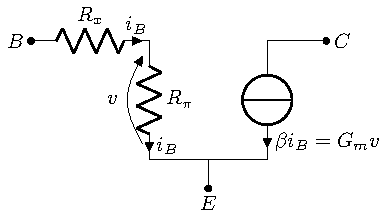
\includegraphics{bjt-due-porte.pdf}%
    \label{fig:bjt-due-porte}
\end{figure}
\noindent
In questo modello $r_x$ corrisponde alla resistenza ohmica di base e quindi è un valore costante indipendente dalla polarizzazione, fornito dal costruttore. Viceversa $R_\pi$, dipende da considerazioni della fisica dello stato solido. RIcordando che i condensatori sono considerati dei cortocircuiti, la linea di alimentazione viene assimilata alla massa e sostituendo il transistor con il suo modello equivalente, il circuito diventerà:
\begin{figure}[H]%
    \centering
    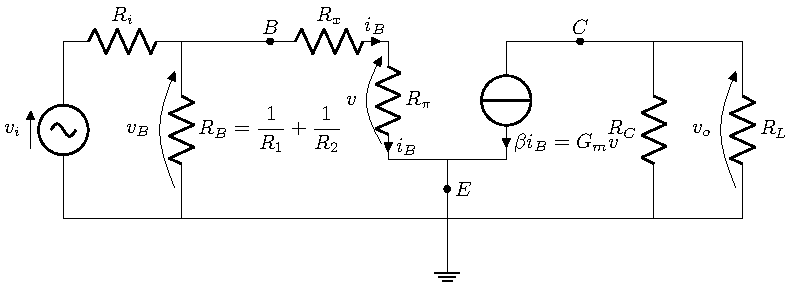
\includegraphics{bjt-piccoli-segnali-due-porte.pdf}%
    \label{fig:bjt-piccoli-segnali-due-porte}
\end{figure}
Solitamente il parametro principale a cui si è interessati è il guadagno di tensione ottenuto dal rapporto tra la tensione in uscita ed in entrata:
\begin{gather*}
    A=\displaystyle\frac{v_o}{v_i}
\end{gather*}
\subsection{Modello a parametri H}
Mentre il modello $\pi$-ibrido si presta ad uno studio dell'amplificatore anche alle alte frequenze, se l'analisi è limitata alle medie frequenze, il modello più utilizzato è quello a parametri h. Normalmente l'amplificatore a transistor si può presentare attraverso tre configurazioni fondamentali, quella che consideriamo è quella a emettitore comune:
\begin{figure}[H]%
    \centering
    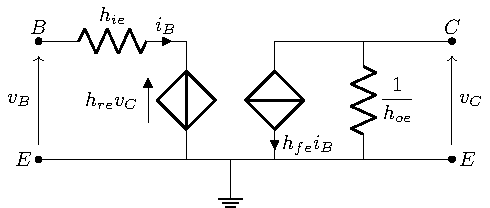
\includegraphics{bjt-parametri-h.pdf}%
    \label{fig:bjt-parametri-h}
\end{figure}
La $i$ al pedice indica input, la $r$ reverse, ed indica che la maglia di uscita controlla in qualche modo la maglia di ingresso. La $f$ sta 
per forward, ed indica che la maglia in entrata controlla la maglia in uscita. Mentre $o$ indica output. 
In generale i parametri H vengono forniti dal fabbricante. 
Per ritornare al caso due-porte sbilanciato si assegnano i seguenti valori ai parametri H:
\begin{gather*}
    h_{ie}=R_x+R_{\pi}\\
    h_{fe}=\beta\\
    h_{oe}=0\\
    h_{re}=0
\end{gather*}
\newpage
\section{Filtri}
\subsection{Filtri del I ordine}
\subsubsection{Filtro Passa-Basso Passivo}
Se prendiamo il segnale sul condensatore C, da un circuito RC serie, otterremo la seguente funzione di trasferimento:
\begin{gather*}
    H(s)=\displaystyle\frac{V_C(s)}{E(s)}=\frac{\displaystyle\frac{1}{sC}}{\frac{1}{sC}+R}=\frac{1}{1+sCR}=\frac{1}{RC\left(s+\displaystyle\frac{1}{RC}\right)}
\end{gather*}
Andiamo a studiarne la risposta in frequenza che si ottiene sostituendo alla variabile $s$ della funzione di rete la quantità immaginaria $j\omega$:
\begin{gather*}
    H(j\omega)=\frac{1}{RC\left(j\omega+\displaystyle\frac{1}{RC}\right)}
\end{gather*}
Questa avrà come modulo e fase:
\begin{gather*}
    |H(j\omega)|=\displaystyle\frac{\displaystyle1}{RC\sqrt{\displaystyle\omega^2+\left(\frac{1}{RC}\right)^2}}\\
    \varphi(\omega)=\arctan\left(-\omega RC\right)
\end{gather*}
Avremo quindi che per \textbf{frequenze basse} $\omega->0$, il valore di $H(j\omega)$ è vicino a 1, il segnale passa quasi inalterato.\\
Invece per \textbf{frequenze alte} $\omega->\infty$, il valore di $H(j\omega)$ tende a 0 e il segnale viene attenuato.\\
Definiamo poi la pulsazione di taglio, come quel particolare valore della pulsazione, che indicheremo con $\omega_t$ tale che:
\begin{gather*}
    H(\omega_t)=\frac{1}{\sqrt{2}}
\end{gather*}
Otteniamo quindi, in virtù del modulo:
\begin{gather*}
    \displaystyle\frac{1}{RC\sqrt{\omega_t^2+\left(\displaystyle\frac{1}{RC}\right)^2}}=\frac{1}{\sqrt2}\\
    \omega_t^2+\left(\displaystyle\frac{1}{RC}\right)^2=2\left(\frac{1}{RC}\right)^2\\
    \omega_t=\displaystyle\frac{1}{RC}\tageq
\end{gather*}
Andando a sostituire nella funzione di trasferimento:
\begin{gather*}
    H(s)=\frac{\omega_t}{(s+\omega_t)}
\end{gather*}
Ricordando che in un circuito serie RC il prodotto RC è pari alla costante di tempo del circuito, possiamo dire che la pulsazione di taglio, è pari all'inverso della costante di tempo. In corrispondenza della pulsazione di taglio, la fase assume il valore:
\begin{gather*}
    \varphi(\omega_t)=\arctan\left(-\displaystyle\frac{1}{RC}RC\right)=\arctan(-1)=-\frac{\pi}{4}
\end{gather*}
Distinguiamo il seguente andamento di modulo e fase:
\begin{figure}[H]%
    \centering
    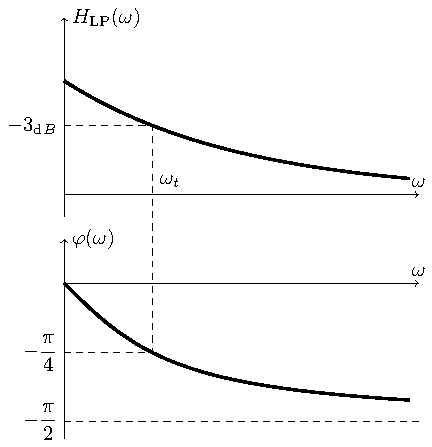
\includegraphics{passa-basso-primo-ordine.pdf}%
\end{figure}
\newpage
\subsubsection{Filtro Passa-Basso Attivo}
Una realizzazione di un \textbf{filtro attivo Passa-Basso} del I ordine è realizzabile attraverso il seguente circuito:
\begin{figure}[H]%
    \centering
    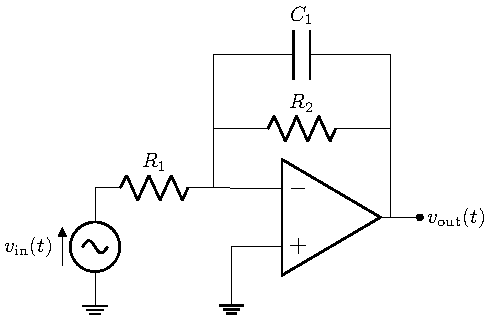
\includegraphics{passa-basso-primo-ordine-attivo.pdf}%
\end{figure}
\noindent
Quest'ultimo avrà la seguente funzione di trasferimento:
\begin{gather*}
    H(s)=-\frac{G_1}{sC_1+G_2}=\frac{\frac{G_1}{C_1}}{s+\frac{G_2}{C_1}}=-\frac{\omega_t}{s+\omega_t}
\end{gather*}
Con $\omega_t=\frac{G_1}{C_1}$ ponendo $G_1=G_2$\\
L'unica differenza con il filtro Passa-Basso passivo infatti sarà solo il segno, che non altererà l'andamento del modulo, mentre causerà un opposizione di fase.
\subsubsection{Filtro Passa-Alto Passivo}
Consideriamo la seguente funzione di trasferimento:
\begin{gather*}
    H(s)=1-H_{LP}(s)= \frac{s}{s+\omega_t}
\end{gather*}
Il comportamento del filtro passa-basso viene così invertito, corrispondendo a un \textbf{filtro Passa-Alto} che esprimiamo con il pedice HP. Andiamo a studiarne la risposta in frequenza che si ottiene sostituendo alla variabile $s$ della funzione di rete la quantità immaginaria $j\omega$:
\begin{gather*}
    H(j\omega)=\frac{j\omega}{j\omega+\omega_t}
\end{gather*}
Questa avrà come modulo e fase:
\begin{gather*}
    |H_{\mathrm{HP}}(\omega)|=\displaystyle\frac{\omega}{\sqrt{\omega^2+\omega_t^2}}\tageq\\
    \varphi(\omega)=\arctan\left(\displaystyle\frac{\omega}{\omega_t}\right)\tageq
\end{gather*}
Avremo quindi che per \textbf{frequenze basse} $\omega->0$, il valore di $H(j\omega)$ tende a 0 e il segnale viene attenuato.\\
Invece per \textbf{frequenze alte} $\omega->\infty$, il valore di $H(j\omega)$ è vicino a 1, il segnale passa quasi inalterato.\\
Ricordando che in un circuito serie RC il prodotto RC è pari alla costante di tempo del circuito, possiamo dire che la pulsazione di taglio, è pari all'inverso della costante di tempo. In corrispondenza della pulsazione di taglio, la fase assume il valore:
\begin{gather*}
    \varphi(\omega_t)=\arctan\left(\displaystyle\frac{1}{RC}RC\right)=\arctan(1)=\frac{\pi}{4}
\end{gather*}
Distinguiamo il seguente andamento di modulo e fase:
\begin{figure}[H]%
    \centering
    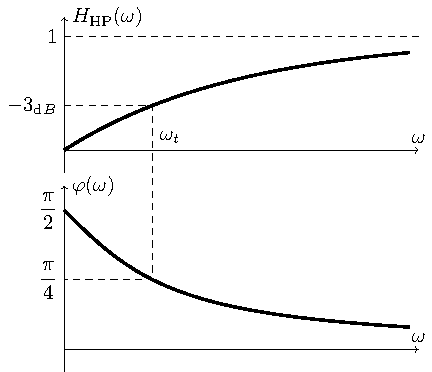
\includegraphics{passa-alto-primo-ordine.pdf}%
\end{figure}
\newpage
\subsubsection{Filtro Passa-Alto Attivo}
Una realizzazione di un \textbf{filtro attivo Passa-Alto} del I ordine è realizzabile attraverso il seguente circuito:
\begin{figure}[H]%
    \centering
    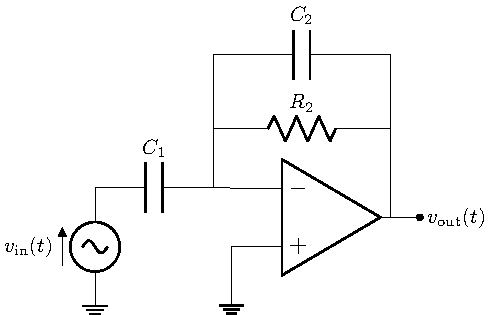
\includegraphics{passa-alto-primo-ordine-attivo.pdf}%
\end{figure}
\noindent
Quest'ultimo avrà la seguente funzione di trasferimento:
\begin{gather*}
    H(s)=-\frac{C_1}{C_2}\frac{s}{s+\frac{G_1}{C_2}}=-\frac{s}{s+\omega_t}
\end{gather*}
Con $\omega_t=\frac{G_1}{C_2}$ e ponendo $C_1=C_2$\\
L'unica differenza con il filtro Passa-Alto passivo infatti sarà solo il segno, che non altererà l'andamento del modulo, mentre causerà un opposizione di fase.
\subsection{Filtri del II ordine}
\subsubsection{Filtro Passa-Banda Passivo}
Se prendiamo il segnale sul resistore R, di un circuito serie R-L-C otterremo la seguente funzione di trasferimento in tensione:
\begin{gather*}
    H_{\mathrm{BP}}(s)=\displaystyle\frac{V_R(s)}{V_i(s)}=\frac{R}{R+\displaystyle\frac{1}{sC}+sL}=\frac{sCR}{sCR+1+s^2LC}=\frac{sCR}{LC\left(\displaystyle s^2+\frac{R}{L}s+\frac{1}{LC}\right)}\\
    H_{\mathrm{BP}}(s)=\displaystyle\frac{sR}{\displaystyle L(s^2+\frac{R}{L}s+\frac{1}{LC})}=\frac{Bs}{(s^2+Bs+\omega_0^2)}
\end{gather*}
Dove $B=\frac{R}{L}$ e $\omega_0=\frac{1}{\sqrt{LC}}$\\
Andiamo a studiarne la risposta in frequenza che si ottiene sostituendo alla variabile $s$ della funzione di rete la quantità immaginaria $j\omega$:
\begin{gather*}
    H(j\omega)=\frac{Bj\omega}{(-\omega^2+Bj\omega+\omega_0^2)}
\end{gather*}
Questa avrà come modulo e fase:
\begin{gather*}
    |H(j\omega)|=\displaystyle\frac{\omega B}{\sqrt{(\omega_0^2-\omega^2)^2+(\omega B)^2}}\tageq\\
    \varphi(\omega)=\arctan\left(\frac{\omega_0^2-\omega^2}{\omega B}\right)
\end{gather*}
Avremo quindi che per \textbf{frequenze basse} $\omega->0$, il valore di $H(j\omega)$ tende a 0 e il segnale viene attenuato.\\
A \textbf{frequenza di risonanza} $\omega=\omega_0$, il valore di $H(j\omega)$ è massimo, quindi il segnale passa quasi inalterato.\\
Invece per \textbf{frequenze alte} $\omega->\infty$, il valore di $H(j\omega)$ tende a 0 e il segnale viene attenuato.\\
Per quanto riguarda l'andamento della fase:
\begin{gather*}
    \varphi(0)=\frac{\pi}{2}\\
    \varphi(\omega_0)=0\\
    \varphi(\infty)=-\frac{\pi}{2}
\end{gather*}
Quindi $\omega_0$ rappresenta \textbf{la pulsazione di risonanza}, cioè quel valore della pulsazione, che rende il circuito come se fosse resistivo puro (si annullano le reattanze capacitiva e induttiva).\\
Distinguiamo il seguente andamento di modulo e fase:
\begin{figure}[H]%
    \centering
    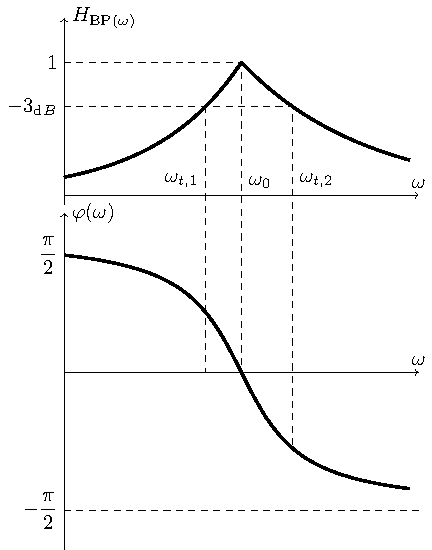
\includegraphics[height=6cm, width=6cm]{passa-banda.pdf}%
\end{figure}
\subsubsection{Filtro Passa-Basso Passivo}
Se prendiamo il segnale sul Condensatore C, di un circuito serie R-L-C otterremo la seguente funzione di trasferimento in tensione:
\begin{gather*}
    H(s)= \frac{\frac{1}{sC}}{sL+R+\frac{1}{sC}}=\frac{1}{s^2LC+sRC+1}=\frac{1}{LC(s^2+\frac{R}{L}s+\frac{1}{LC})}=\frac{\omega_0}{(s^2+Bs+\omega_0^2)}
\end{gather*}
Dove $B=\frac{R}{L}$ e $\omega_0=\frac{1}{\sqrt{LC}}$\\
Andiamo a studiarne la risposta in frequenza che si ottiene sostituendo alla variabile s della funzione di rete la quantità immaginaria $j\omega$:
\begin{gather*}
    H(j\omega)=\frac{\omega_0}{(-\omega^2+Bj\omega+\omega_0^2)}
\end{gather*}
Questa avrà come modulo e fase:
\begin{gather*}
    |H(j\omega)|=\frac{\omega_0}{\sqrt{(B\omega)^2+(\omega_0^2-\omega^2)^2}}\\
     \varphi(\omega)=\begin{cases}
        \arctan\left(\displaystyle-\frac{\strut \omega B}{\omega_0^2-\omega^2}\right)&\omega\leq\omega_0\\
        \arctan\left(\displaystyle-\frac{\strut \omega B}{\omega_0^2-\omega^2}\right)-\pi&\omega>\omega_0
    \end{cases}
\end{gather*}
Vogliamo determinare il valore dell'omega di taglio:
\begin{gather*}
    \displaystyle\frac{\omega_0^2}{\sqrt{(\omega_0^2-\omega_t^2)^2+(\omega_t B)^2}}=\frac{1}{\sqrt2}\\
    \omega_t=\displaystyle\sqrt{\frac{-(B^2-2\omega_0^2)+\sqrt{(B^2-2\omega_0^2)^2+4\omega_0^2}}{2}}\tageq
\end{gather*}
Si analizza ora la frequenza corrispondente al valore di massimo, si cerca questo valore trovando il valore minimo del denominatore:
\begin{gather*}
    \displaystyle\frac{\df}{\df\omega}\left[{{(\omega_0^2-\omega^2)^2+(\omega B)^2}}\right]=0\\
    2B^2\omega_m-4\omega_m(\omega_0^2-\omega^2)=0\\
    \omega_m=\displaystyle\frac{4\omega_0^2-2B^2}{4}\tageq
\end{gather*}
Avremo quindi che per \textbf{frequenze basse} $\omega \to 0$, il valore di $H(j\omega)$ tende a 1, quindi il segnale passa quasi inalterato.\\  
A \textbf{frequenza di risonanza} $\omega=\omega_0$, il valore di $H(j\omega)$ è ancora elevato, quindi il segnale passa con massimo guadagno.\\  
Invece per \textbf{frequenze alte} $\omega \to \infty$, il valore di $H(j\omega)$ tende a 0 e il segnale viene attenuato.\\  
Per quanto riguarda l'andamento della fase:  
\begin{gather*}
    \varphi(0)=0\\
    \varphi(\omega_0)=-\frac{\pi}{2}\\
    \varphi(\infty)=-\pi
\end{gather*}
\begin{figure}[H]%
    \centering
    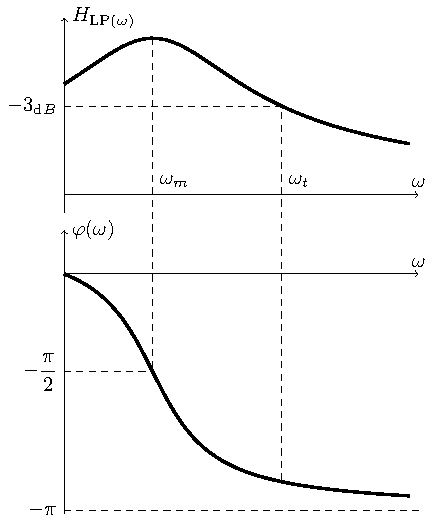
\includegraphics{passa-basso-secondo-ordine.pdf}%
\end{figure}
\subsubsection{Filtro Passa-Alto Passivo}
Se prendiamo il segnale sull'induttore L, di un circuito serie R-L-C otterremo la seguente funzione di trasferimento in tensione:
\begin{gather*}
    H_{L}(s)=\displaystyle\frac{s^2}{s^2+\displaystyle s\frac{R}{L}+\frac1{LC}}=\frac{s^2}{s^2+sB+\omega_0^2}=H_{\mathrm{HP}}(s)\\
\end{gather*}
Dove $B=\frac{R}{L}$ e $\omega_0=\frac{1}{\sqrt{LC}}$\\
Andiamo a studiarne la risposta in frequenza che si ottiene sostituendo alla variabile $s$ della funzione di rete la quantità immaginaria $j\omega$:
\begin{figure}[H]%
    \centering
    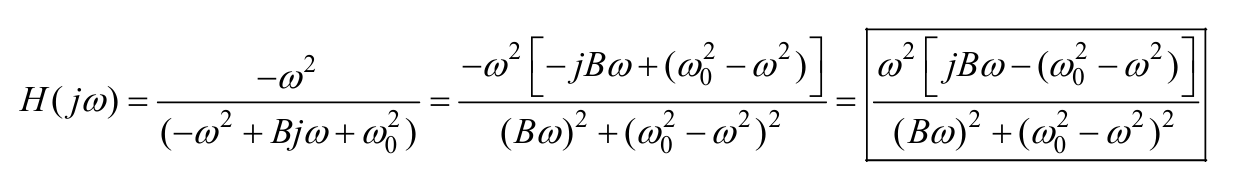
\includegraphics[width=14cm, height=2cm]{immagine_2025-02-19_174324742.png}%
    \label{fig:Funzione di trasferimento}
\end{figure}
\noindent
Questa avrà come modulo e fase:
\begin{gather}
    |H(\omega)|=\displaystyle\frac{\omega^2}{\sqrt{(\omega_0^2-\omega^2)^2+(\omega B)^2}}\\
\end{gather}
\begin{gather}
    \varphi(\omega)=\begin{cases}
        \arctan\left(\displaystyle-\frac{\strut \omega B}{\omega_0^2-\omega^2}\right)+\pi&\omega\leq\omega_0\\
        \arctan\left(\displaystyle-\frac{\strut \omega B}{\omega_0^2-\omega^2}\right)&\omega>\omega_0
    \end{cases}
\end{gather}
Vogliamo determinare il valore dell'omega di taglio:
\begin{gather}
    \omega_t=\displaystyle\sqrt{\frac{(B^2-2\omega_0^2)+\sqrt{(B^2-2\omega_0^2)^2+4\omega_0^2}}{2}}
\end{gather}
Si analizza ora la frequenza corrispondente al valore di massimo, si cerca questo valore trovando il valore minimo del denominatore:
\begin{gather*}
    \displaystyle\frac{\df}{\df \omega}\left[\frac{B^2\omega^2}{\omega^4}+\frac{\omega_0^4}{\omega^4}-2\frac{\omega_0^2\omega^2}{\omega^4}+\frac{\omega^4}{\omega^4}\right]=0\\
    \omega_m=\displaystyle\sqrt{\frac{4\omega_0^4}{4\omega_0^2-2B^2}}\tageq
\end{gather*}
Avremo quindi che per \textbf{frequenze basse} $\omega \to 0$, il valore di $H(j\omega)$ tende a 0, quindi il segnale viene attenuato.\\  
A \textbf{frequenza di risonanza} $\omega=\omega_0$, il valore di $H(j\omega)$ è massimo, quindi il segnale passa quasi inalterato.\\  
Invece per \textbf{frequenze alte} $\omega \to \infty$, il valore di $H(j\omega)$ tende a 1 e il segnale passa quasi inalterato.\\  
Per quanto riguarda l'andamento della fase:  
\begin{gather*}
    \varphi(0) = \pi\\
    \varphi(\omega_0) = \frac{\pi}{2}\\
    \varphi(\infty) = 0
\end{gather*}
\begin{figure}[H]%
    \centering
    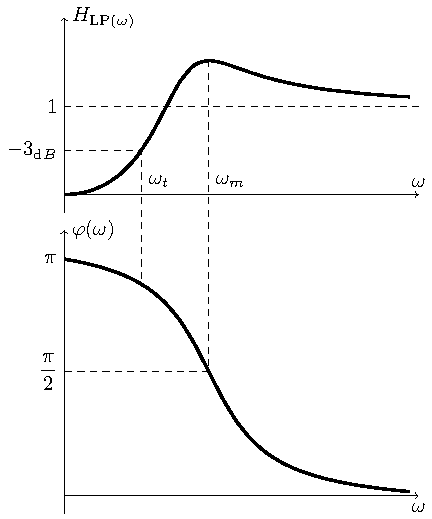
\includegraphics{passa-alto-secondo-ordine.pdf}%
\end{figure}
\subsubsection{Filtro Elimina-Banda Passivo}
Se prendiamo il segnale somma della tensione sull'induttore L e sul condensatore C, di un circuito serie R-L-C otterremo la seguente funzione di trasferimento in tensione:
\begin{gather*}
    H(s)=\frac{\frac{1}{sC}+sL}{sL+R+\frac{1}{sC}}=\frac{1+s^2LC}{s^2LC+sRC+1}=\frac{LC(s^2+\frac{1}{LC})}{LC(s^2+\frac{R}{L}s+\frac{1}{LC})}\\
    H(s)=\frac{s^2+\omega_0^2}{(s^2+Bs+\omega_0^2)}
\end{gather*}
Dove $B=\frac{R}{L}$ e $\omega_0=\frac{1}{\sqrt{LC}}$\\
Andiamo a studiarne la risposta in frequenza che si ottiene sostituendo alla variabile s della funzione di rete la quantità immaginaria $j\omega$:
\begin{gather*}
    H(s)=\frac{\omega_0^2-\omega^2}{(-\omega^2+Bj\omega+\omega_0^2)}
\end{gather*}
Questa avrà come modulo e fase:
\begin{gather*}
    |H(j\omega)|=\frac{|\omega_0^2-\omega^2|}{\sqrt{(B\omega)^2+(\omega_0^2-\omega^2)^2}}\\
    \varphi(\omega)=\arctan(\frac{-B\omega}{\omega_0^2-\omega^2})
\end{gather*}
Vogliamo determinare il valore dell'omega di taglio:
\begin{gather*}
    \omega_t=\sqrt{\frac{(B^2+2\omega_0^2)\overset{+}{-}\sqrt{(B^2+2\omega_0^2)^2-4\omega_0^4}}{2}}
\end{gather*}
Avremo quindi che per \textbf{frequenze basse} $\omega \to 0$, il valore di $H(j\omega)$ tende a 1, quindi il segnale passa quasi inalterato.\\  
A \textbf{frequenza di risonanza} $\omega=\omega_0$, il valore di $H(j\omega)$ è minimo, quindi il segnale viene attenuato al massimo.\\  
Invece per \textbf{frequenze alte} $\omega \to \infty$, il valore di $H(j\omega)$ tende a 1 e il segnale passa quasi inalterato.\\  
Per quanto riguarda l'andamento della fase:   
\begin{gather*}
    \varphi(0) = 0\\
    \varphi(\omega_0) = -\frac{\pi}{2}\\
    \varphi(\infty) = -\pi
\end{gather*}
\begin{figure}[H]%
    \centering
    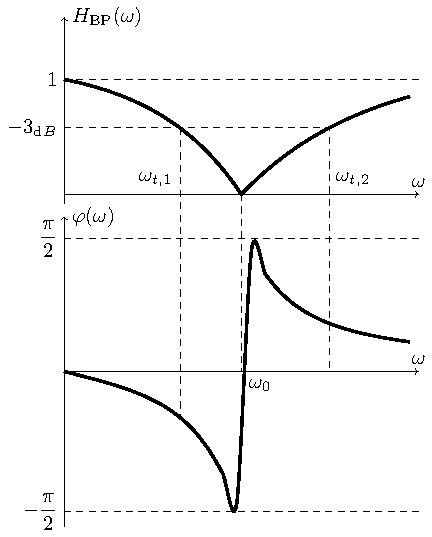
\includegraphics{reiezione-banda}%
\end{figure}
\newpage
\subsubsection{Filtro Passa-Banda Attivo}
Una realizzazione di un \textbf{filtro attivo Passa-Banda} del II ordine è realizzabile attraverso il seguente circuito:
\begin{figure}[H]%
    \centering
    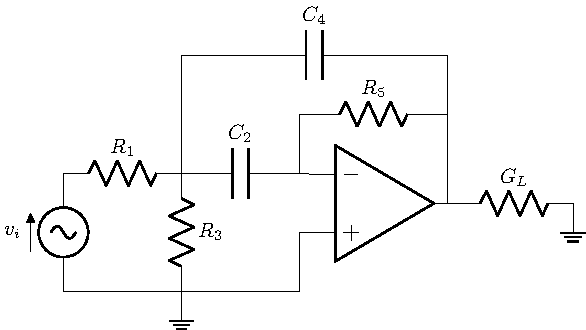
\includegraphics{filtro-attivo-2.pdf}%
\end{figure} 
\noindent
Quest'ultimo avrà la seguente funzione di trasferimento:
\begin{gather*}
    H(s)=\frac{Bs}{s^2+Bs+\omega_0^2}
\end{gather*}
\clearpage
\end{document}
